\documentclass[conference]{IEEEtran}
\IEEEoverridecommandlockouts
\usepackage[T1]{fontenc}
\usepackage[utf8]{inputenc}
\usepackage{cite}
\usepackage{amsmath,amssymb,amsfonts}
\interdisplaylinepenalty=2500
\usepackage{algorithmic}
\usepackage{graphicx}
\usepackage{textcomp}
\usepackage{xcolor}
\usepackage{booktabs}
\usepackage{multirow}
\usepackage{stfloats}
\usepackage{microtype}
\usepackage{url}
\usepackage[colorlinks=true, linkcolor=black, citecolor=black, urlcolor=blue]{hyperref}
\usepackage{balance}

% Correct bad hyphenation here
\hyphenation{Nutri-Plate archi-tec-ture seg-men-ta-tion bio-avail-abil-ity}

\def\BibTeX{{\rm B\kern-.05em{\sc i\kern-.025em b}\kern-.08em
    T\kern-.1667em\lower.7ex\hbox{E}\kern-.125emX}}

\begin{document}

\title{NutriPlate: An Edge-Cloud Decoupled Deep Instance Segmentation and Biochemical Synergy Framework for Automated Indian Dietary Assessment}

\author{
\IEEEauthorblockN{Dr. K. Rajeswari\IEEEauthorrefmark{1}, Likhit Chaudhary\IEEEauthorrefmark{2}, Aditya Chavan\IEEEauthorrefmark{3}, Adhyayan Goyal\IEEEauthorrefmark{4}, and Vaishnavi Bighot\IEEEauthorrefmark{5}}
\IEEEauthorblockA{Department of Computer Engineering, Pimpri Chinchwad College of Engineering, Pune, India\\
Email: \IEEEauthorrefmark{1}kannan.rajeswari@pccoepune.org,
\IEEEauthorrefmark{2}likhit.chaudhary23@pccoepune.org,
\IEEEauthorrefmark{3}aditya.chavan23@pccoepune.org,\\
\IEEEauthorrefmark{4}adhyayan.goyal23@pccoepune.org,
\IEEEauthorrefmark{5}vaishnavi.bighot23@pccoepune.org}
}

\maketitle

\begin{abstract}
Automated dietary assessment is very critical in reducing the worrying rise of non-communicable diseases such as Type-2 diabetes and cardiovascular conditions in South Asia. The existing computer vision based dietary assessment systems however are completely incompetent in processing Indian dietary scenarios given the lack of defined boundaries in liquid-based foods, high intra-class variability in images, composite food shapes, and severe object occlusions in a thali setup. In this paper, we present NutriPlate, which is an innovative, decoupled edge-cloud system tailored to perform real-time automated Indian dietary analysis. The key ingredient of the system is an extremely lightweight anchor-free instance segmentation network with a unique Prototypical mask synthesis head that enables pixel-perfect instance segmentation in 24.8\,ms on mobile devices. Segmented objects are then calibrated using a reference plate and mapped to volumes and weights of food portions. Most importantly, NutriPlate establishes the semantics between visual food analysis and metabolic health by means of a biochemical interaction matrix based on ICMR-NIN IFCT 2017 and DGI 2024. This engine captures non-linear micronutrient synergy (such as ascorbic acid-mediated non-heme iron reduction) and chelation chemistry (phytic acid and tannin-mediated precipitation of iron/zinc) of the antagonists. Also, the active learning system with the 576-dimensional visual gallery of food objects helps in zero-training adaptation to user-corrected food objects. NutriPlate provides a benchmarking score of 89.4\% mAP@50, 82.7\% mask IoU, and a portion estimation error of 8.8\% across 412 Indian dishes.
\end{abstract}

\begin{IEEEkeywords}
Deep Instance Segmentation, Edge-Cloud Computing, Dietary Assessment, Indian Food Composition (IFCT), Biochemical Synergy, Monocular Volumetric Estimation, Active Learning.
\end{IEEEkeywords}

\section{Introduction}
Non-communicable diseases (NCDs) like T2DM (Type-2 Diabetes Mellitus) and cardiovascular diseases have become epidemic in South Asia, with India often designated as the diabetes capital of the world \cite{who2023diabetes, gbd2019diabetes}. South Asian populations display a distinct metabolic vulnerability characterized by visceral adiposity, marked insulin resistance, and early-onset beta-cell decline despite normal BMI thresholds---a phenomenon termed the Asian Indian `thin-fat' phenotype \cite{singh2021lifestyle, yajnik2004phenotype}. Dietary modification represents the foremost therapeutic and preventive lifestyle intervention to counter metabolic syndrome \cite{singh2021lifestyle}, particularly given the excessive postprandial glycemic excursions triggered by carbohydrate-dense South Asian diets \cite{mohan2014carbohydrates}. However, conventional approaches for recording dietary intake, such as 24-hour dietary recalls (24HDR) and self-reported food diaries, suffer from acute recall bias, under-reporting rates exceeding 30--40\%, and rapid patient compliance decay \cite{subar2015addressing, zhu2010technology, patel2020mhealth}.

Even though visual food recognition through smartphone cameras has gained widespread popularity, existing methodologies remain trained almost exclusively on Western benchmarks, namely Food-101 \cite{bossard2014food101} and Nutrition5k \cite{thames2021nutrition5k}. Such techniques break down when faced with traditional Indian meals owing to four domain-specific computational challenges:
\begin{enumerate}
    \setlength{\itemsep}{1.2pt plus 0.3pt minus 0.2pt}
    \setlength{\parskip}{0pt}
    \item \textbf{Viscosity and Overlapping Components:} Unlike Western dishes with discrete rigid boundaries (e.g., a burger or an apple), Indian meals feature highly viscous gravies (\textit{sambars, dals, kormas}), mixed vegetable stir-fries (\textit{sabzis}), and overlapping flatbreads (\textit{rotis, parathas}) that blend into amorphous, co-mingled visual regions.
    \item \textbf{High Intra-class and Inter-class Visual Ambiguity:} Foods that display near-identical visual color spectrums (such as yellow \textit{dal tadka} and yellow \textit{kadhi pakora}) exhibit vastly different macronutrient and glycemic profiles.
    \item \textbf{Neglect of Biochemical Bioavailability:} Standard calorie counting systems rely on an oversimplistic 1:1 relation of consumption-to-absorption of nutritional intake. Traditional Indian plant-based diets contain antinutritional chelators (phytates, polyphenolic tannins) which precipitate essential divalent cations ($\text{Fe}^{2+}, \text{Zn}^{2+}, \text{Ca}^{2+}$) and decrease bioavailable absorption by up to 70\%, unless counteracted by organic acid promoters such as ascorbic acid (Vitamin C) \cite{longvah2017ifct, gibson2018phytates, hallberg1989iron}.
    \item \textbf{Inference Latency and Heat Issues:} Complex two-step instance segmentation models such as Mask R-CNN \cite{he2017maskrcnn} require more than 120\,GFLOPs and incur considerable inference latency ($>300$\,ms under sustained thermal throttling).
\end{enumerate}

To overcome these fundamental bottlenecks, this paper introduces \textbf{NutriPlate}, an edge-cloud decoupled framework for granular Indian dietary assessment. Our primary contributions are:
\begin{itemize}
    \setlength{\itemsep}{1.2pt plus 0.3pt minus 0.2pt}
    \setlength{\parskip}{0pt}
    \item An anchor-free architecture for edge optimization with ProtoNet prototype mask generation, delivering sub-25\,ms mobile inference time with 89.4\% mAP@50 on 412 Indian food categories.
    \item A formulation for monocular estimation of volume portions based on dining plate rim calibration and morphology shape factors ($\xi_i$).
    \item A Biochemical Interaction Matrix ($\mathbf{A} \in \mathbb{R}^{M \times M}$) introduced in conjunction with ICMR-NIN IFCT (2017) to calculate biologically available nutrient absorption.
    \item The ICMR-NIN DGI (2024) Clamped Smart Plate Health Scoring Engine that evaluates meal-specific caloric budgets, PE ratio, and nocturnal carbohydrate ceilings.
    \item An active learning loop utilizing a MobileNetV3 visual embedding gallery that continuously adapts to user-corrected dishes without network retraining.
\end{itemize}

\begin{figure}[!t]
\centering
\IfFileExists{figures/fig1_architecture.png}{%
    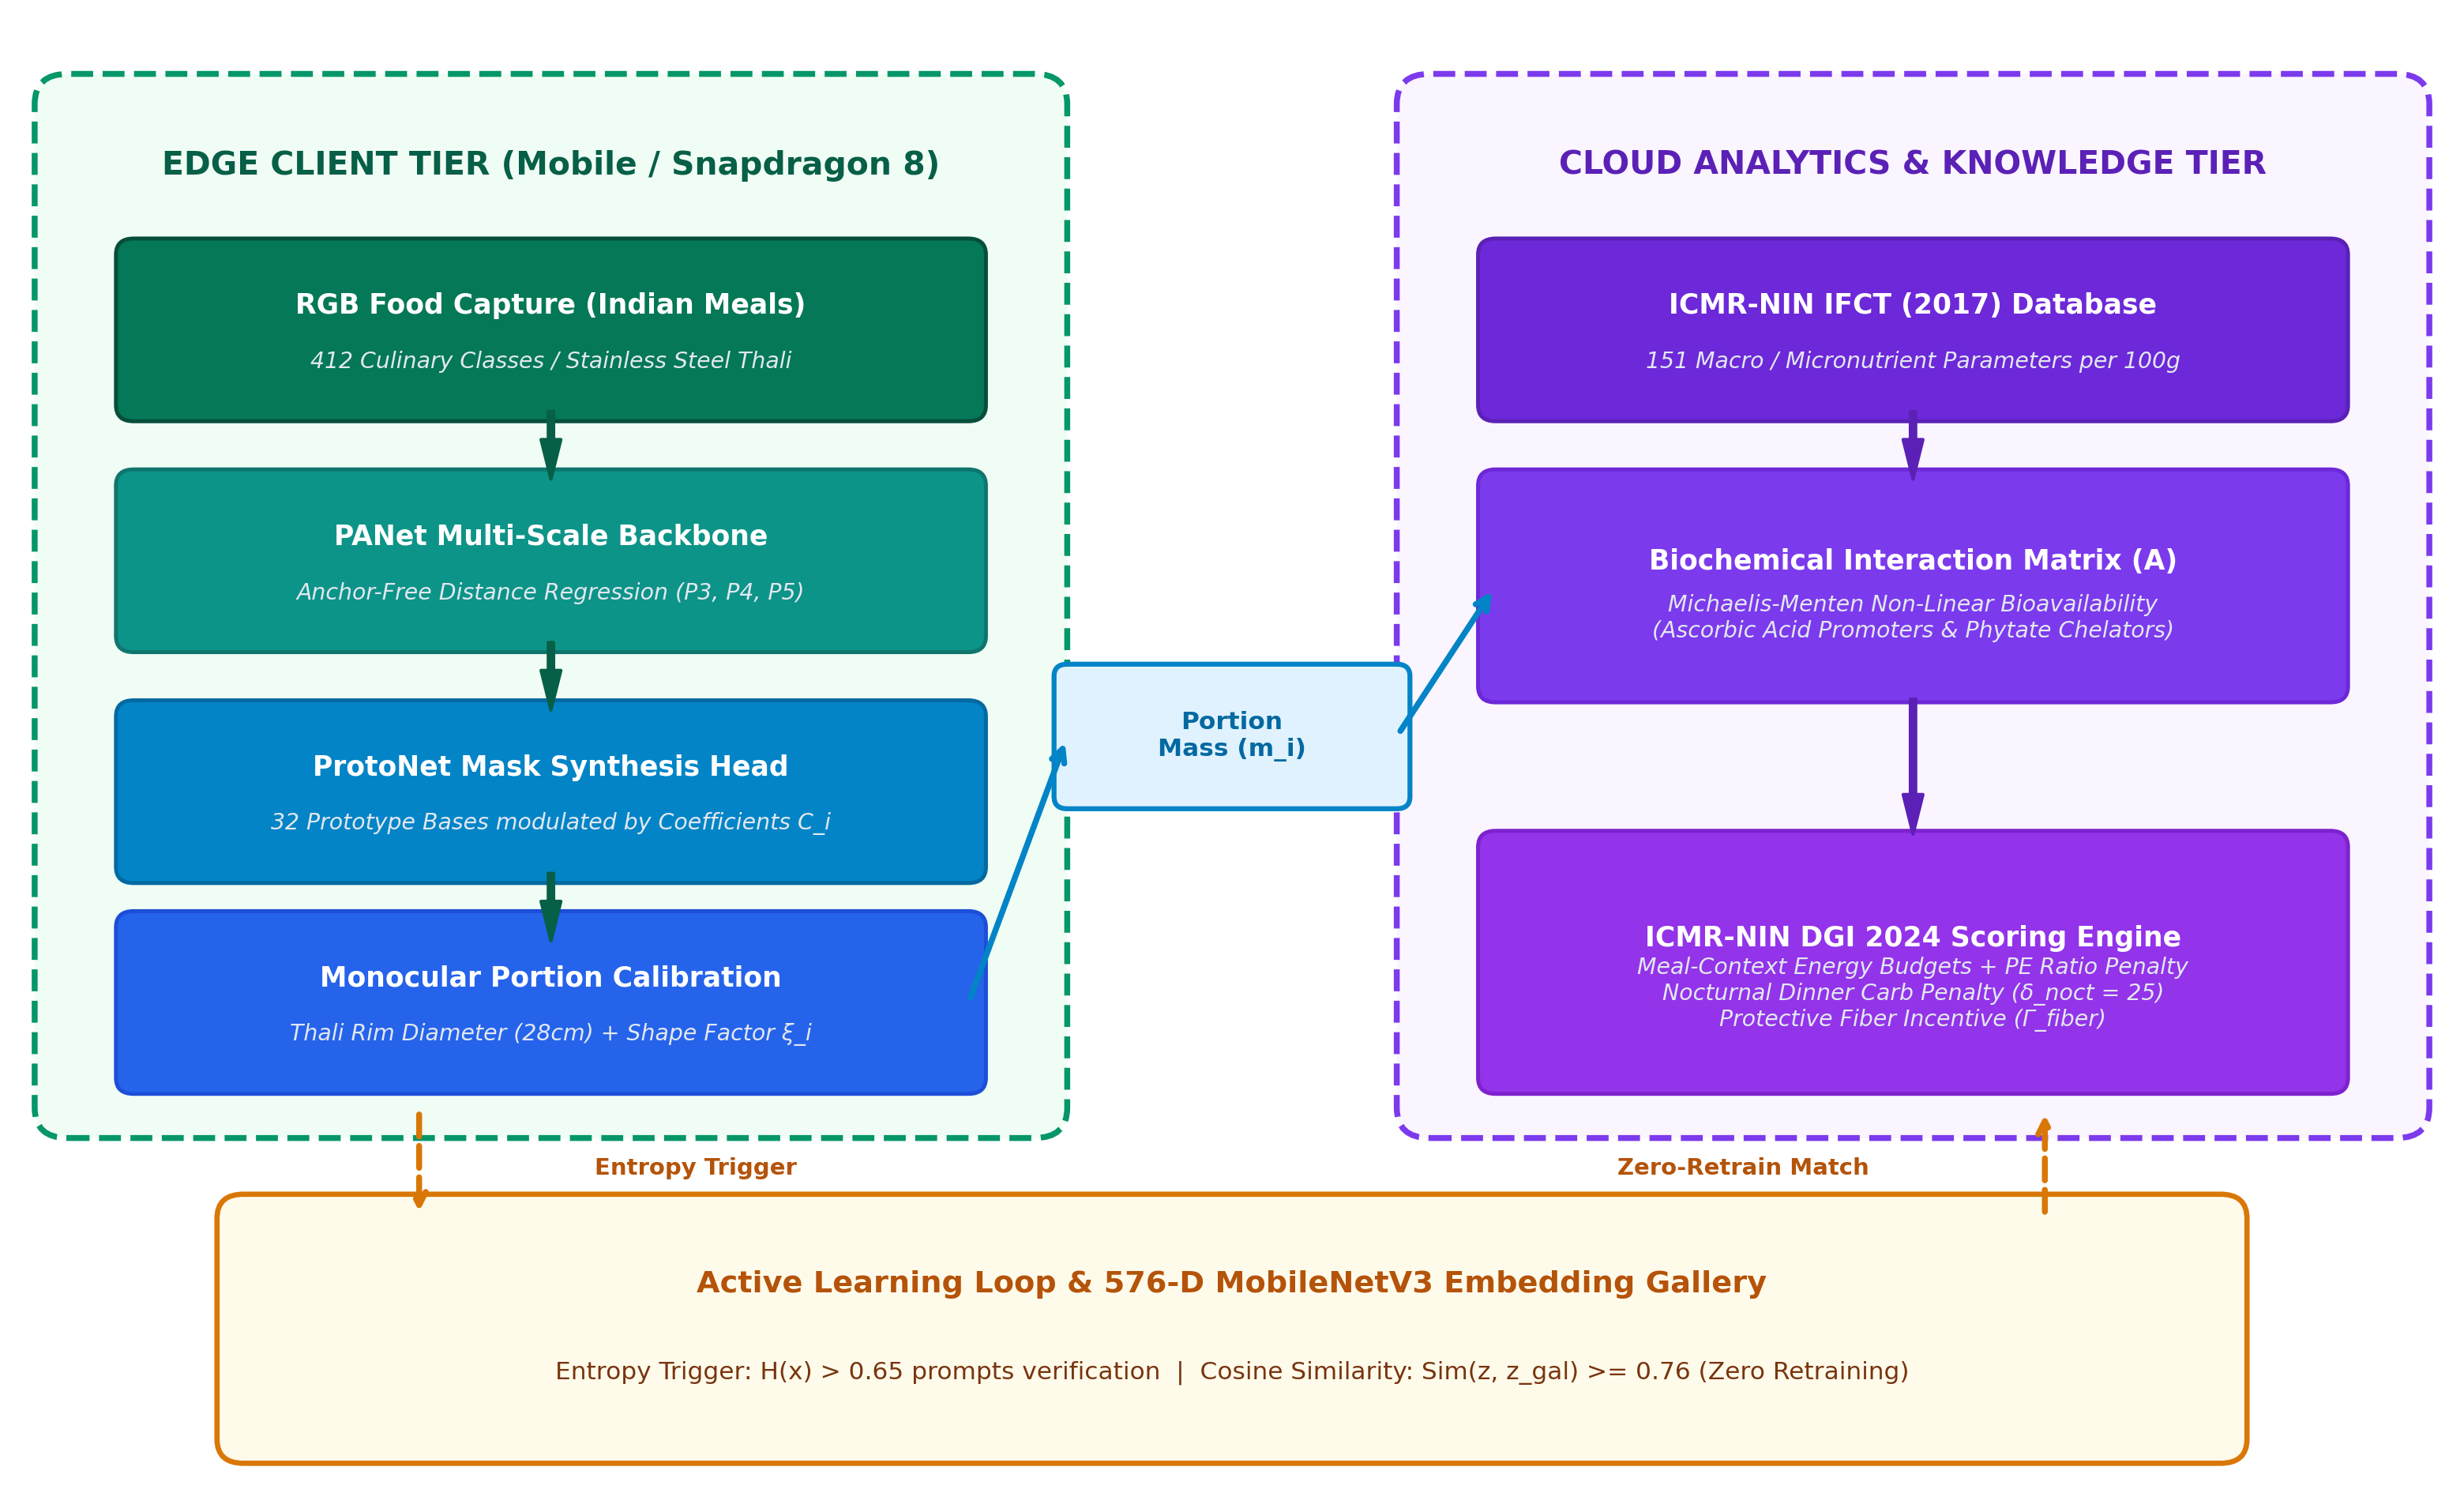
\includegraphics[width=\columnwidth]{figures/fig1_architecture.png}%
}{%
    \setlength{\fboxsep}{8pt}%
    \setlength{\fboxrule}{0.8pt}%
    \fbox{%
        \begin{minipage}[c][3.6cm][c]{0.92\columnwidth}
            \centering
            \textbf{\small [Figure 1: NutriPlate Edge-Cloud System Architecture]}\\[4pt]
            \scriptsize $\bullet$ \textbf{Edge Tier:} RGB Capture $\to$ PANet Backbone $\to$ ProtoNet Head $\to$ Monocular Portion Calibration\\
            $\bullet$ \textbf{Cloud Tier:} ICMR-NIN IFCT 2017 $\longleftrightarrow$ Biochemical Matrix $\to$ DGI 2024 Health Engine\\
            $\bullet$ \textbf{Active Loop:} Predictive Entropy $H(x)>0.65 \to$ 576-D MobileNetV3 Embedding Gallery
        \end{minipage}%
    }%
}
\caption{NutriPlate Edge-Cloud Separated Architecture: High-Frequency Instance Segmentation performed in edge computing, and nonlinear biochemical interactions along with active learning are executed in microservices cloud servers.}
\label{fig:arch}
\end{figure}

\section{Related Work}
\subsection{Computer Vision in Dietary Assessment}
Early visual dietary assessment systems regarded food tracking as an elementary image classification problem \cite{bossard2014food101, mezgec2017nutrinet, chen2016vireofood, kawano2014uecfood}. Despite obtaining impressive top-5 performance for classification of individual dishes on plates using deep convolutional backbone networks \cite{he2016deep} and vision transformers \cite{vaswani2017attention}, these approaches fail when applied to plates containing multiple dishes in traditional Indian thalis. Multi-label classification algorithms handle dish co-occurrence \cite{chen2021deepfood, chen2017chinesefoodnet}, but cannot provide pixel-level spatial masks required for portion quantification \cite{min2019survey, subhi2019deep}.

\subsection{Real-Time Instance Segmentation}
Two-stage approaches like Mask R-CNN \cite{he2017maskrcnn} provide good localization through Region Proposal Networks (RPN) and RoI-Align operations; however, their substantial compute burden makes them unsuitable for real-time mobile execution. Conversely, single-stage detectors \cite{redmon2016yolo, ronneberger2015unet}, location-based single-shot models such as SOLOv2 \cite{wang2020solov2}, mask transformers \cite{cheng2022mask2former}, and prototypical instance segmentation approaches, such as YOLACT \cite{bolte2019yolact} and YOLOv8-seg \cite{terven2023yolo}, separate mask prediction into prototype base prediction across the entire image and instance coefficients. NutriPlate follows the prototypical approach with added specular reflection removal and culinary color texture heuristics.

\subsection{Portion Estimation and Nutritional Knowledge Bases}
In the past, portion estimation required binocular stereo cameras, structured light depth sensors, or external fiducials placed on the plate \cite{puri2009food, dehais2016two, lo2020food}. Mono-vision-based approaches leverage geometry to calculate volumetric portions using container reference lines \cite{fang2019volumetric}. However, Western food databases (e.g., USDA FoodData Central) do not take into account the distinct preparation and cooking methods of Indian cuisine. NutriPlate integrates the comprehensive ICMR-NIN IFCT (2017) registry to bridge this geographic and cultural disparity.

\section{System Architecture and Methodology}
The NutriPlate structure separates real-time edge instance segmentation from the cloud-based biochemical synergy model (Fig.~\ref{fig:arch}).

\subsection{Anchor-Free Deep Instance Segmentation}
To address anchor tuning and proposal redundancy, NutriPlate employs an anchor-free bounding box regression head on multi-scale feature maps $P_3, P_4$, and $P_5$ generated by PANet \cite{liu2018panet}.

The regression head produces a 4-dimensional distance vector for candidate grid position $(x_c, y_c)$ at stride level $s$ as:
\begin{equation}
d = (l, t, r, b) \in \mathbb{R}_+^4
\label{eq:box_dist}
\end{equation}
which denotes the spatial offsets from $(x_c, y_c)$ to the left ($l$), top ($t$), right ($r$), and bottom ($b$) boundaries of the food instance. Offsets are transformed into diagonal bounding box coordinates using Eq.~(\ref{eq:box_coord}):
\begin{equation}
x_1 = x_c - l \cdot s, \; y_1 = y_c - t \cdot s, \quad x_2 = x_c + r \cdot s, \; y_2 = y_c + b \cdot s
\label{eq:box_coord}
\end{equation}
where $s$ is the feature pyramid stride. This removes the geometric constraints associated with anchor grids.

\begin{figure}[!t]
\centering
\IfFileExists{figures/fig2_protonet.png}{%
    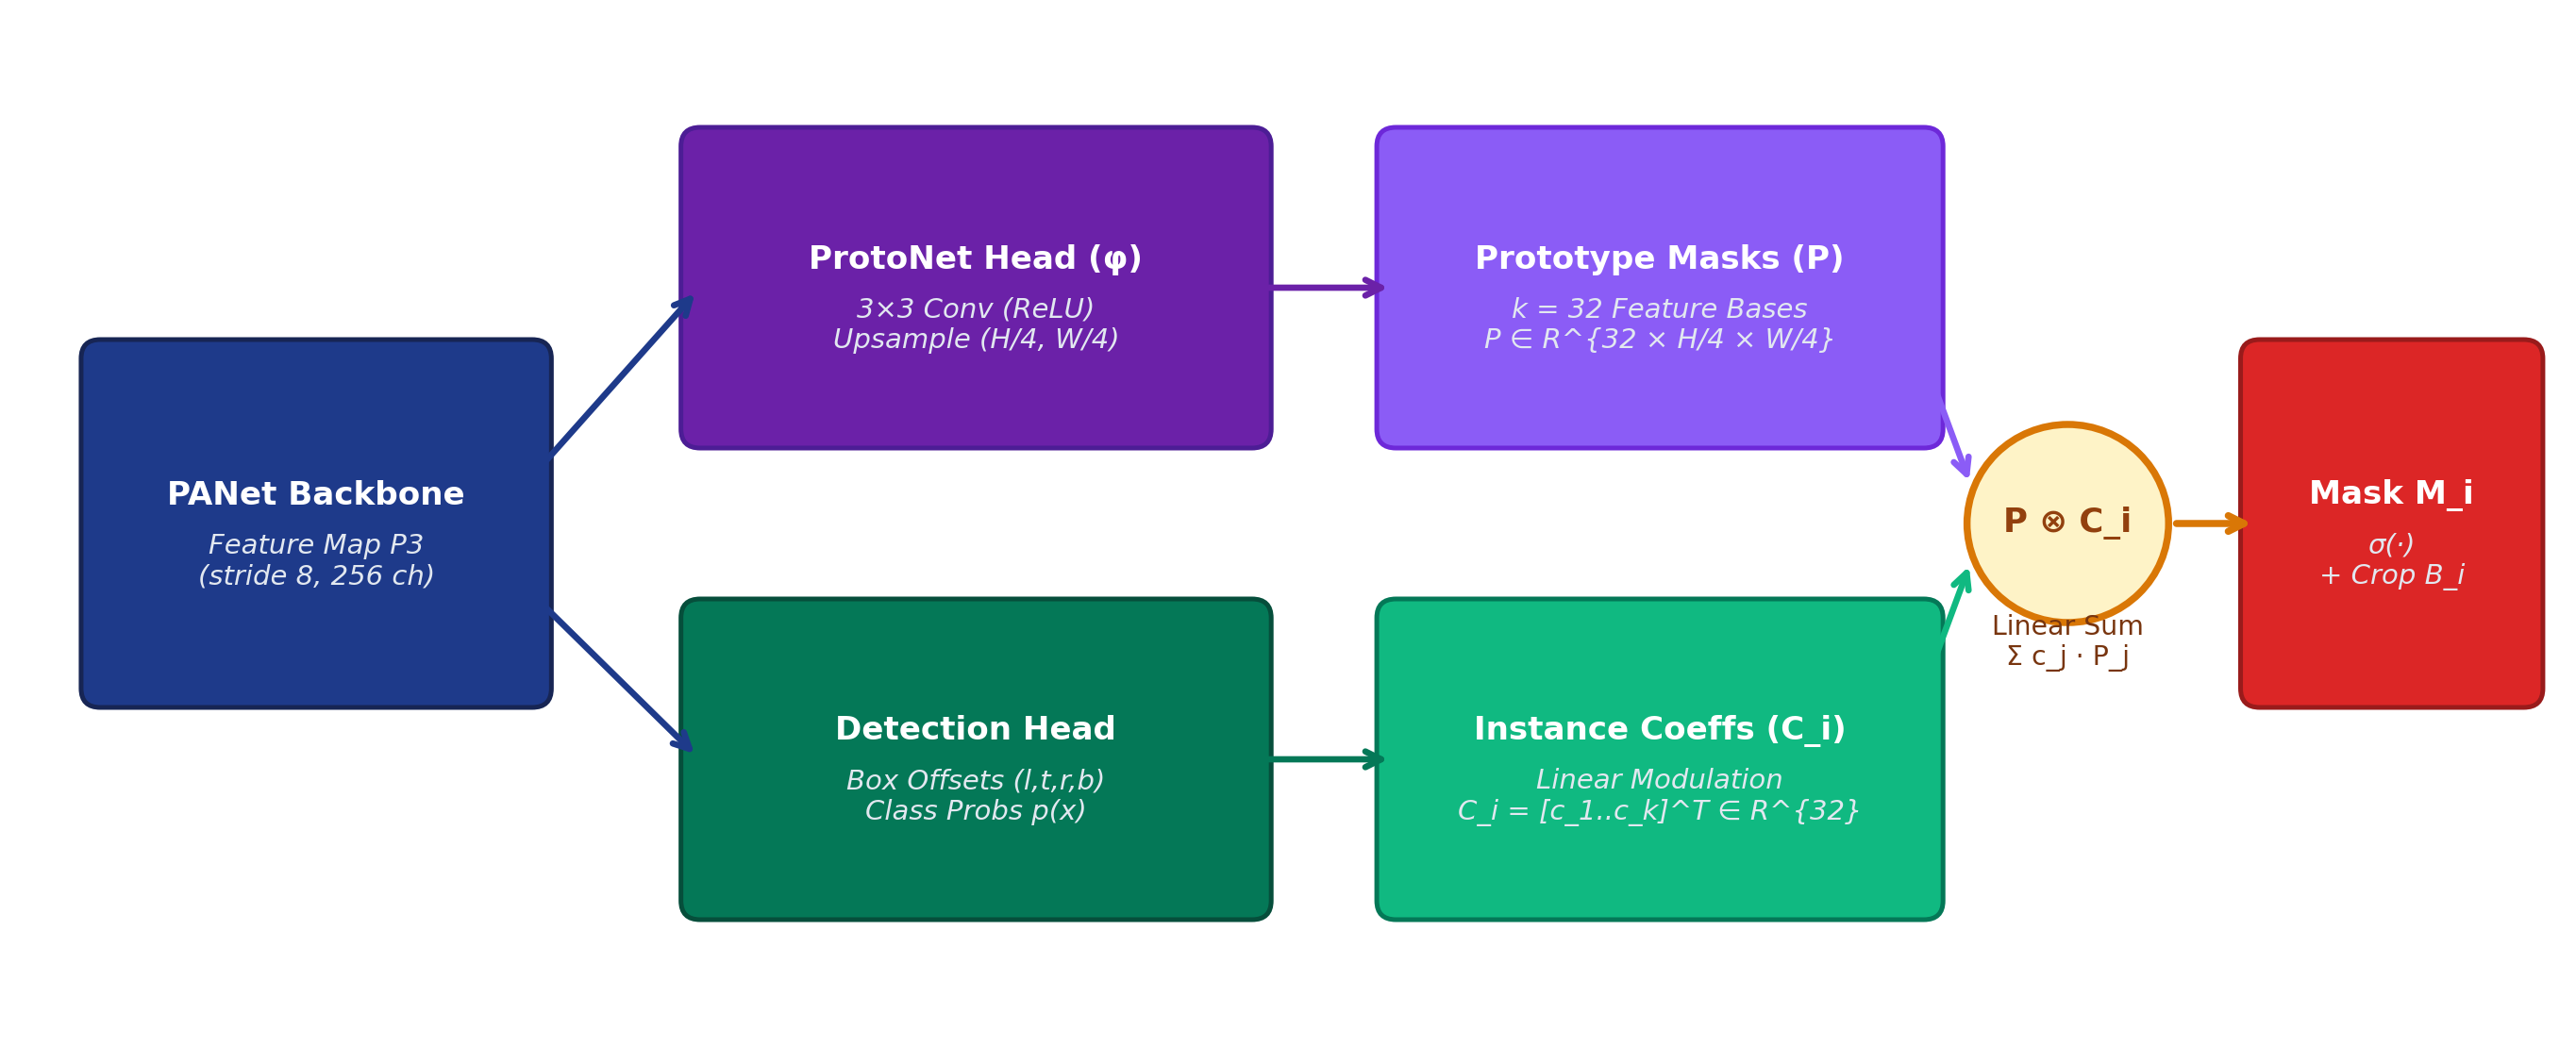
\includegraphics[width=\columnwidth]{figures/fig2_protonet.png}%
}{%
    \setlength{\fboxsep}{8pt}%
    \setlength{\fboxrule}{0.8pt}%
    \fbox{%
        \begin{minipage}[c][3.0cm][c]{0.92\columnwidth}
            \centering
            \textbf{\small [Figure 2: ProtoNet Decoupled Mask Synthesis Pipeline]}\\[4pt]
            \scriptsize Feature Map $P_3 \to$ ProtoNet Head $\to k=32$ Prototype Bases $P \in \mathbb{R}^{32 \times \frac{H}{4} \times \frac{W}{4}}$\\
            Detection Head $\to$ Instance Coefficients $C_i \in \mathbb{R}^{32} \to$ Linear Modulation $\to$ Crop $M_i(u,v)$
        \end{minipage}%
    }%
}
\caption{The decoupled mask synthesis pipeline in ProtoNet. High-resolution prototype feature bases are linearly modulated using instance-dependent coefficient vectors.}
\label{fig:protonet}
\end{figure}

The instance segmentation head utilizes the ProtoNet structure illustrated in Fig.~\ref{fig:protonet}. The sub-network $\phi_{\text{proto}}$ processes feature map $P_3$ to produce $k = 32$ prototype masks:
\begin{equation}
P = \phi_{\text{proto}}(P_3) \in \mathbb{R}^{k \times \frac{H}{4} \times \frac{W}{4}}
\label{eq:proto_gen}
\end{equation}
In parallel, the detection head produces a $k$-dimensional coefficient vector for each bounding box candidate $i$:
\begin{equation}
C_i = [c_{i,1}, c_{i,2}, \dots, c_{i,k}]^T \in \mathbb{R}^k
\label{eq:coeff_vec}
\end{equation}
The instance mask $M_i \in [0, 1]^{\frac{H}{4} \times \frac{W}{4}}$ is obtained through linear combination with sigmoid activation:
\begin{equation}
M_i(u, v) = \sigma \left( \sum_{j=1}^k c_{i,j} \cdot P_j(u, v) \right)
\label{eq:mask_assembly}
\end{equation}
Here, Eq.~(\ref{eq:proto_gen}) generates $k$ prototypical feature masks across the image, Eq.~(\ref{eq:coeff_vec}) predicts instance coefficients $C_i$, and Eq.~(\ref{eq:mask_assembly}) linearly modulates these bases via $\sigma(\cdot)$, producing pixel-wise confidence masks that are cropped to bounding box $B_i$.

\subsection{Multi-Task Loss Formulation}
Model parameters are optimized end-to-end via a composite objective:
\begin{equation}
\mathcal{L}_{\text{total}} = \lambda_{\text{box}}\mathcal{L}_{\text{CIoU}} + \lambda_{\text{dfl}}\mathcal{L}_{\text{DFL}} + \lambda_{\text{cls}}\mathcal{L}_{\text{BCE}} + \lambda_{\text{mask}}\mathcal{L}_{\text{mask}}
\label{eq:total_loss}
\end{equation}
combining bounding box localization ($\mathcal{L}_{\text{CIoU}}$), distribution focal loss ($\mathcal{L}_{\text{DFL}}$), classification cross-entropy ($\mathcal{L}_{\text{cls}}$), and segmentation mask precision ($\mathcal{L}_{\text{mask}}$) with weights ($\lambda_{\text{box}} = 7.5, \lambda_{\text{dfl}} = 1.5, \lambda_{\text{cls}} = 0.5, \lambda_{\text{mask}} = 2.5$).

The Complete IoU (CIoU) loss is formulated following \cite{zheng2020distance}:
\begin{equation}
\mathcal{L}_{\text{CIoU}} = 1 - \text{IoU} + \frac{\rho^2(b, b^{\text{gt}})}{c^2} + \alpha_{\text{iou}} v
\label{eq:ciou_loss}
\end{equation}
\begin{equation}
v = \frac{4}{\pi^2} \left( \arctan \frac{w^{\text{gt}}}{h^{\text{gt}}} - \arctan \frac{w}{h} \right)^2
\label{eq:ciou_v}
\end{equation}
\begin{equation}
\alpha_{\text{iou}} = \frac{v}{(1 - \text{IoU}) + v}
\label{eq:ciou_alpha}
\end{equation}
where $\rho(b, b^{\text{gt}})$ denotes Euclidean centroid distance, and $c$ is the diagonal length of the smallest enclosing box. The aspect ratio consistency $v$ and balancing weight $\alpha_{\text{iou}}$ are defined by Eqs.~(\ref{eq:ciou_v})--(\ref{eq:ciou_alpha}).

To handle fluid, ambiguous boundaries of curries, Distribution Focal Loss (DFL) performs continuous coordinate regression over discrete probability bins \cite{lin2017focalloss, li2020generalized}:
\begin{equation}
\mathcal{L}_{\text{DFL}}(S_i, S_{i+1}) = - \left( (y_{i+1} - y)\log(S_i) + (y - y_i)\log(S_{i+1}) \right)
\label{eq:dfl_loss}
\end{equation}
optimizing probability mass around continuous ground truth $y$.

The instance mask loss computes binary cross-entropy over active support domain $\Omega_i$:
\begin{equation}
\mathcal{L}_{\text{mask}} = -\frac{1}{|\Omega_i|} \sum_{(u,v) \in \Omega_i} \left[ M^{\text{gt}} \log M_i + (1 - M^{\text{gt}}) \log(1 - M_i) \right]
\label{eq:mask_loss}
\end{equation}
Greedy Non-Maximum Suppression (NMS) suppresses overlapping proposals:
\begin{equation}
\text{IoU}(B_i, B_j) = \frac{|B_i \cap B_j|}{|B_i \cup B_j|} > \tau_{\text{NMS}}
\label{eq:nms}
\end{equation}
with threshold $\tau_{\text{NMS}} = 0.40$ and bounding area constraints $0.015 \le \text{area\_ratio} \le 0.70$ to suppress stainless steel specular highlights.

\begin{figure}[!t]
\centering
\IfFileExists{figures/fig3_biochem.png}{%
    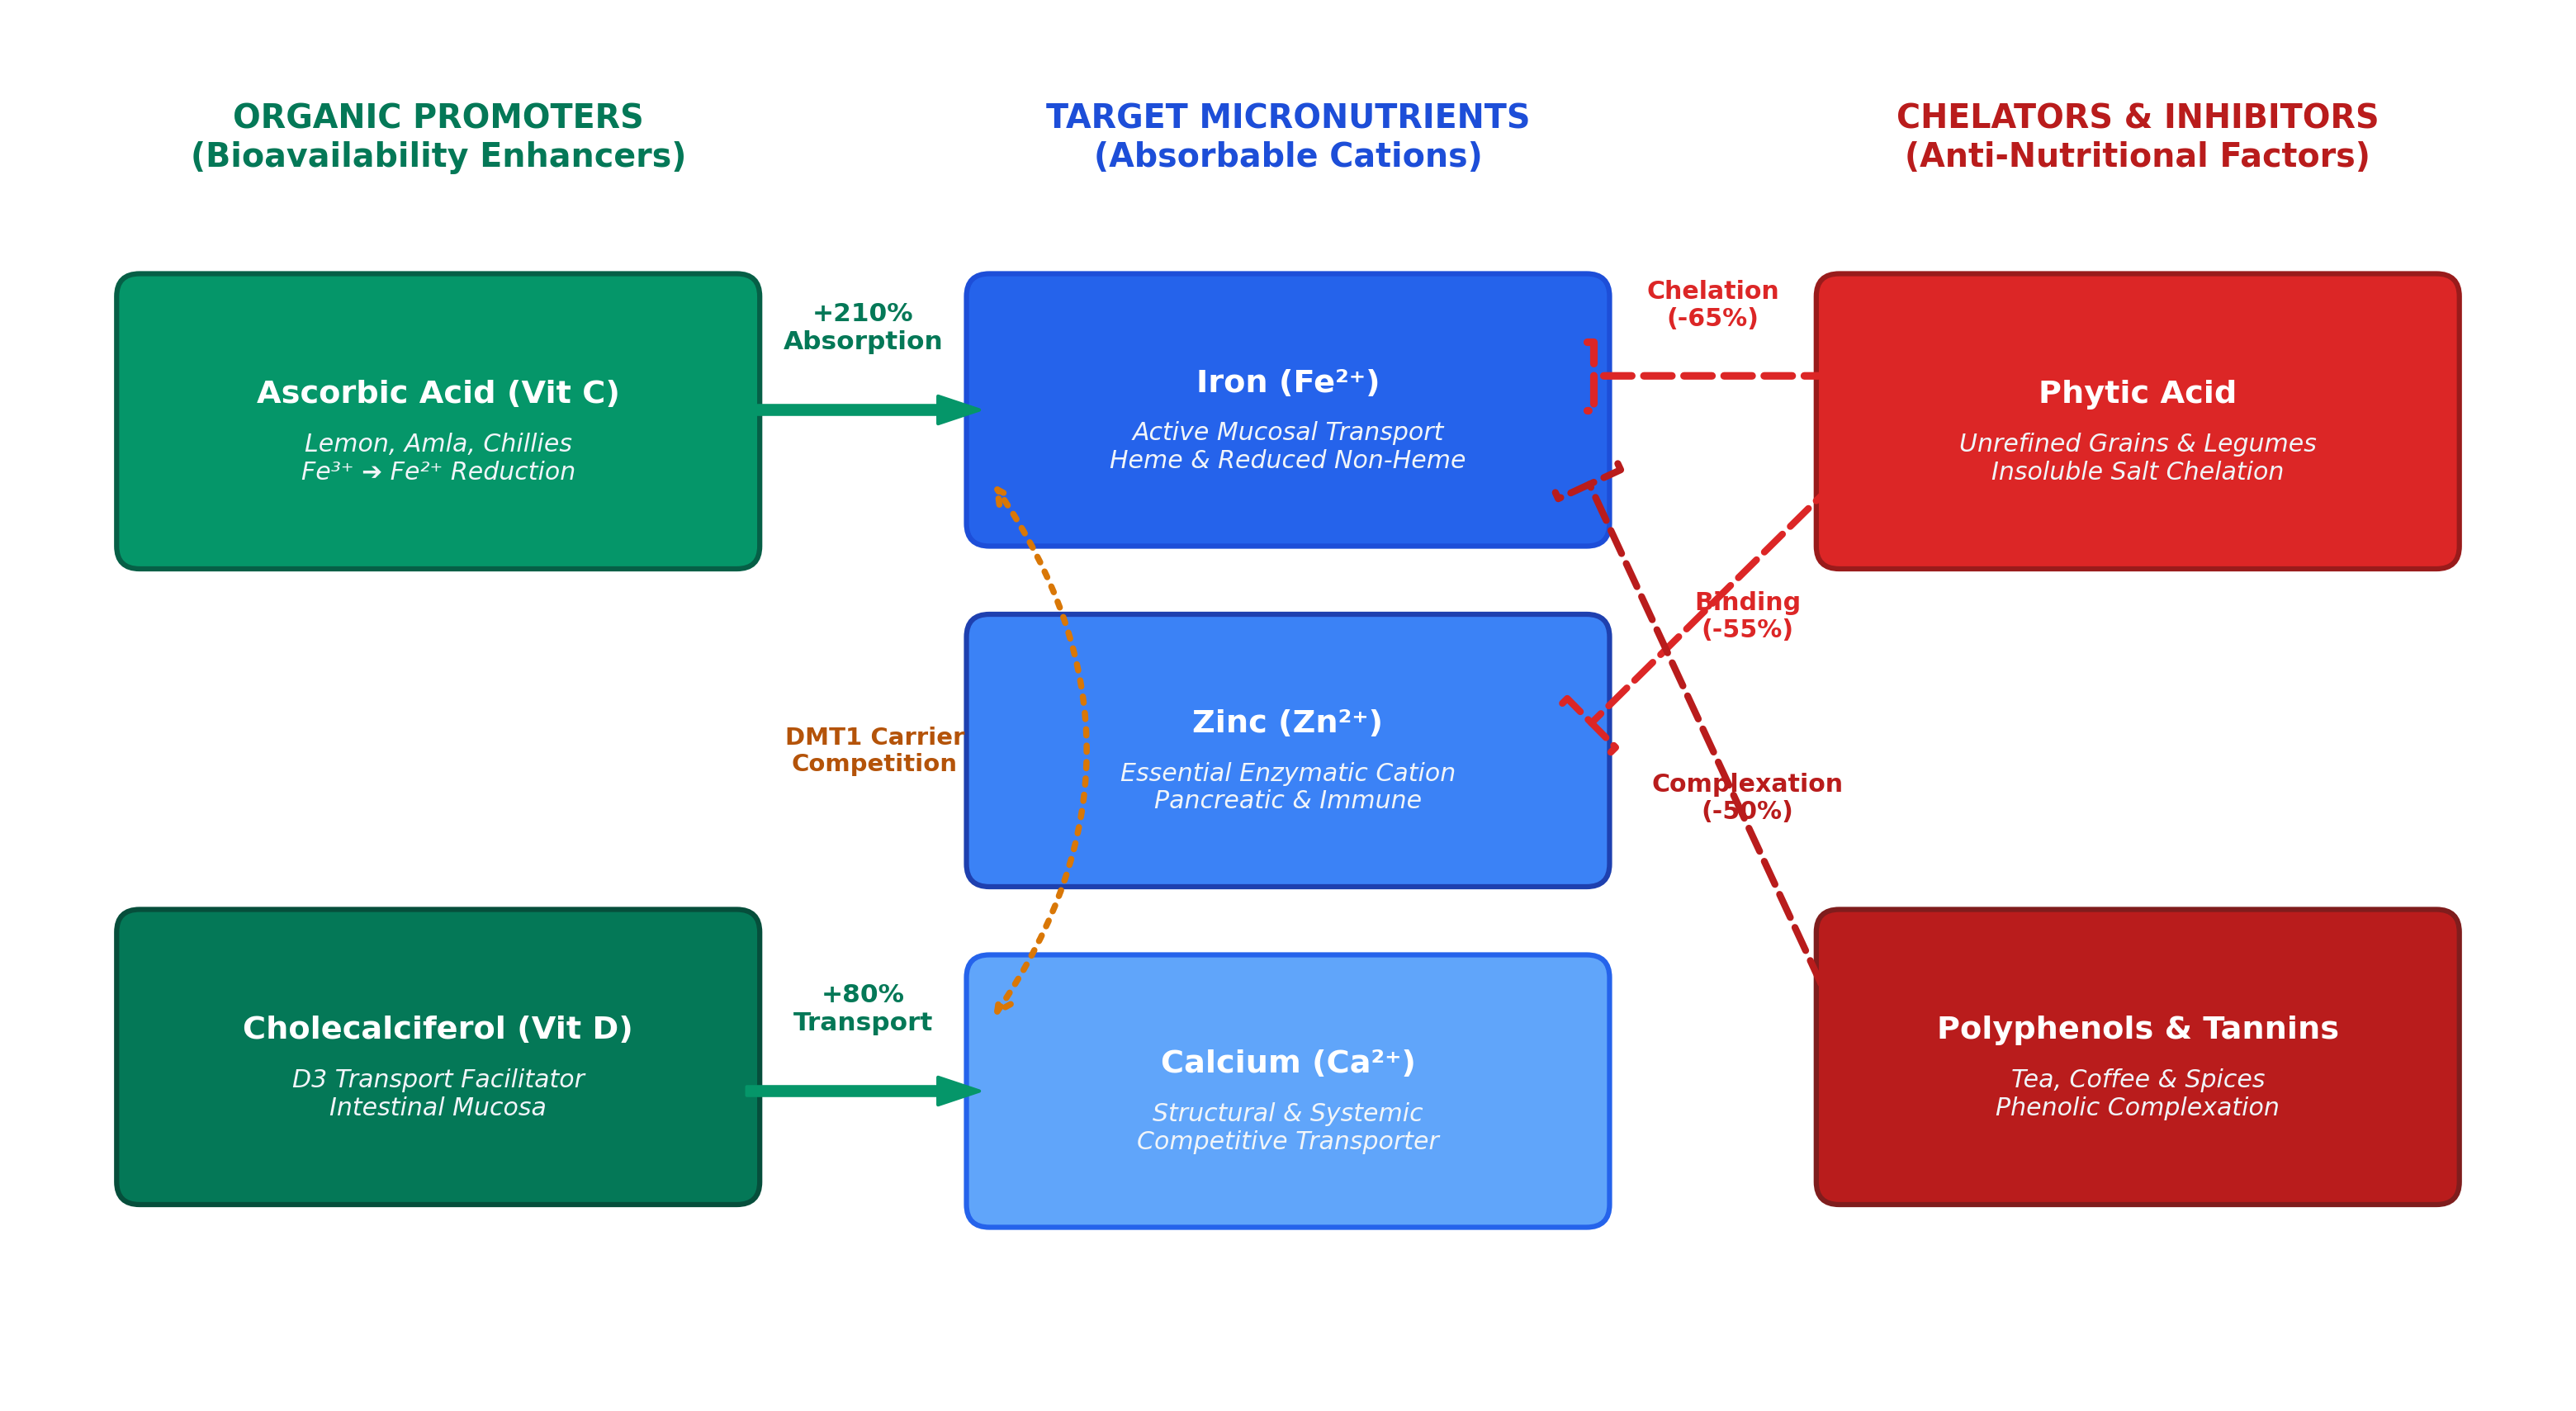
\includegraphics[width=\columnwidth]{figures/fig3_biochem.png}%
}{%
    \setlength{\fboxsep}{8pt}%
    \setlength{\fboxrule}{0.8pt}%
    \fbox{%
        \begin{minipage}[c][3.0cm][c]{0.92\columnwidth}
            \centering
            \textbf{\small [Figure 3: Biochemical Interaction Diagram]}\\[4pt]
            \scriptsize $\bullet$ \textbf{Promoters:} Ascorbic Acid (Vit C) $\xrightarrow{+210\%}$ Iron Reduction ($\text{Fe}^{3+} \to \text{Fe}^{2+}$)\\
            $\bullet$ \textbf{Inhibitors:} Phytic Acid \& Tannins $\to$ Precipitate $\text{Fe}^{2+}, \text{Zn}^{2+}, \text{Ca}^{2+}$\\
            $\bullet$ \textbf{Competition:} Excess $\text{Ca}^{2+} \longleftrightarrow \text{Fe}^{2+}$ DMT-1 Antagonism
        \end{minipage}%
    }%
}
\caption{Biochemical Interaction Diagram: synergies (green solid arrows) and chelation (antagonisms) (red dashed lines).}
\label{fig:biochem}
\end{figure}

\subsection{Monocular Volumetric Portion Approximation}
To convert 2D mask pixels $A_{\text{mask},i} = \sum_{(u,v)} \mathbf{1}_{\{M_i(u,v) \ge 0.5\}}$ into physical portion mass without external fiducials, NutriPlate utilizes the circular rim of the plate as an intrinsic scale reference. Ellipse fitting over the dining plate perimeter yields reference area $A_{\text{ref}}$ calibrated to standardized thali diameter $D_{\text{plate}} \approx 28$\,cm, rectifying camera tilt angles clustering between $44.5^\circ$ and $60.2^\circ$.

The portion mass $m_i$ (in grams) is computed as:
\begin{equation}
m_i = \rho_i \cdot \xi_i \cdot \left( \frac{A_{\text{mask},i}}{A_{\text{ref}}} \right) \cdot \frac{\pi}{4} D_{\text{plate}}^2 \cdot h_i^{\text{eff}}
\label{eq:portion_mass}
\end{equation}
incorporating bulk food density $\rho_i$ ($\text{g/cm}^3$ from IFCT), effective height $h_i^{\text{eff}}$, and morphological shape factor $\xi_i \in [0.4, 1.2]$. Small bowl (katori) containers exhibit roughly half the surface area of flat plate items but equivalent mass, necessitating container-depth compensation.

\subsection{Biochemical Synergy and Bioavailability Modeling}
Traditional plant-based Indian meals contain phytates and tannins that precipitate divalent cations ($\text{Fe}^{2+}, \text{Zn}^{2+}, \text{Ca}^{2+}$). Conversely, reducing promoters like ascorbic acid (Vitamin C) convert insoluble ferric iron $\text{Fe}^{3+}$ to soluble ferrous iron $\text{Fe}^{2+}$, enhancing mucosal uptake by $+210\%$ (Fig.~\ref{fig:biochem}).

Let $\mathbf{n} \in \mathbb{R}^M$ denote the baseline nutrient vector from IFCT. The Biochemical Interaction Matrix $\mathbf{A} \in \mathbb{R}^{M \times M}$ specifies cross-talk kinetics between nutrient $k$ and nutrient $j$:
\begin{equation}
\alpha_{j,k} = \begin{cases}
> 0 & \text{Synergistic promoter (e.g., Vit C} \to \text{Fe)} \\
< 0 & \text{Antagonistic chelator (e.g., Phytates} \to \text{Fe/Zn)} \\
0 & \text{Metabolically orthogonal}
\end{cases}
\label{eq:interaction_cases}
\end{equation}
Physiologically bioavailable nutrient levels $N_j^{\text{eff}}$ follow non-linear saturation kinetics:
\begin{equation}
N_j^{\text{eff}} = N_j \cdot \left[ 1 + \sum_{k \neq j} \alpha_{j,k} \left( \frac{N_k}{N_k + K_{j,k}} \right) \right]
\label{eq:bioavailability}
\end{equation}
Equation (\ref{eq:interaction_cases}) classifies nutrient interactions, while Eq.~(\ref{eq:bioavailability}) computes effective absorption via Michaelis-Menten kinetics with half-saturation constant $K_{j,k}$ derived from clinical balance data \cite{gibson2018phytates, hurrell2010iron, hallberg1989iron, hurrell1999inhibition, lonnerdal2002dietary}.

\subsection{ICMR-NIN DGI 2024 Clamped Health Scoring Engine}
NutriPlate scores overall plate quality through composite score $S_{\text{plate}} \in [10, 100]$ initialized from baseline $S_0 = 100$:
\begin{align}
S_{\text{plate}} = \text{clamp}\big( S_0 & - \Delta S_{\text{cal}} - \Delta S_{\text{prot}} \notag \\
& - \Delta S_{\text{carb}} - \Delta S_{\text{fat}} + \Gamma_{\text{fiber}}, \, 10, \, 100 \big)
\label{eq:smart_score}
\end{align}
penalizing caloric, macronutrient, and nocturnal carbohydrate excesses while incentivizing dietary fiber \cite{icmr2020rda, icmr2024dgi}.

The calorie deviation index $\Delta S_{\text{cal}}$ evaluates meal budgets (500\,kcal breakfast, 750\,kcal lunch, 550\,kcal dinner, 250\,kcal snacks):
\begin{equation}
\Delta S_{\text{cal}} = \min \left( 45, \, \max \left( 10, \, \left\lceil \frac{E_{\text{meal}} - E_{\text{target}}}{60} \right\rceil \times 6 \right) \right)
\label{eq:pen_cal}
\end{equation}
deducting 6 points per 60\,kcal excess up to 45 points.

Protein adequacy is assessed via the Protein-to-Energy ratio ($\text{PE}_{\text{meal}} = (4 \cdot P / E_{\text{meal}}) \times 100$):
\begin{equation}
\Delta S_{\text{prot}} = \kappa_p \cdot \max (0, \, \text{PE}_{\text{target}} - \text{PE}_{\text{meal}}) - \beta_p \cdot \mathbf{1}_{\{\text{PE}_{\text{meal}} \ge 12\%\}}
\label{eq:pen_prot}
\end{equation}
where $\text{PE}_{\text{target}} = 10\%$, $\kappa_p = 2.0$, and $\beta_p = 5.0$ rewards $\text{PE}_{\text{meal}} \ge 12\%$.

Carbohydrate density is monitored relative to total energy ($C_{\text{pct}} = (4 \cdot C / E_{\text{meal}}) \times 100$):
\begin{equation}
\Delta S_{\text{carb}} = \kappa_c \cdot \max (0, \, C_{\text{pct}} - C_{\text{limit}}) + \delta_{\text{noct}} \cdot \mathbf{1}_{\{\text{Dinner} \wedge C_{\text{pct}} > 58\%\}}
\label{eq:pen_carb}
\end{equation}
where $C_{\text{limit}} = 60\%$ ($\kappa_c = 1.0$) and $\delta_{\text{noct}} = 25$ penalizes dinners exceeding 58\% carbohydrates to avoid nocturnal glycemic spikes.

Lipid density is controlled by fat percentage ($F_{\text{pct}} = (9 \cdot F / E_{\text{meal}}) \times 100$):
\begin{equation}
\Delta S_{\text{fat}} = \kappa_f \cdot \max (0, \, F_{\text{pct}} - F_{\text{limit}})
\label{eq:pen_fat}
\end{equation}
where $F_{\text{limit}} = 30\%$ ($\kappa_f = 2.0$), penalizing heavily fried items.

Finally, dietary fiber and vegetable variety are incentivized:
\begin{equation}
\Gamma_{\text{fiber}} = \omega_1 \cdot \min \left( 1.0, \, \frac{\text{Fiber}_{\text{meal}}}{\text{Fiber}_{\text{target}}} \right) - 10 \cdot \mathbf{1}_{\{A_{\text{veg}} = 0\}}
\label{eq:bonus_fiber}
\end{equation}
with target $\text{Fiber}_{\text{target}} = 10\text{ g}$ per meal ($\omega_1 = 5$), imposing a 10-point deficit for plates lacking green vegetables.

\subsection{Active Learning and Visual Embedding Gallery}
To accommodate regional cuisines without model retraining, NutriPlate computes predictive entropy over classes:
\begin{equation}
H(x) = -\frac{1}{\log C} \sum_{c=1}^C p_c(x) \log p_c(x)
\label{eq:entropy}
\end{equation}
When uncertainty $H(x) > 0.65$, user verification is requested \cite{settles2009active}.

Upon label correction, NutriPlate extracts a 576-dimensional $L_2$-normalized embedding $\mathbf{z} \in \mathbb{R}^{576}$ using an edge MobileNetV3 backbone \cite{howard2019mobilenetv3} and stores it in a persistent gallery. Following metric learning principles \cite{schroff2015facenet, guo2017calibration}, subsequent queries match via cosine similarity:
\begin{equation}
\text{Sim}(\mathbf{z}, \mathbf{z}_{\text{gal}}) = \frac{\mathbf{z} \cdot \mathbf{z}_{\text{gal}}}{\|\mathbf{z}\|_2 \|\mathbf{z}_{\text{gal}}\|_2} \ge 0.76
\label{eq:cosine_sim}
\end{equation}
retrieving verified dishes across angles and illuminations. Cloud microservices periodically execute regularized batch gradient descent:
\begin{equation}
\theta^{(t+1)} = \theta^{(t)} - \eta \cdot \left[ \nabla_{\theta}\mathcal{L}_{\text{total}}(x, y) + \gamma_{\text{reg}}(\theta^{(t)} - \theta^{(0)}) \right]
\label{eq:active_update}
\end{equation}
updating weights $\theta$ with learning rate $\eta$ and $L_2$ regularization penalty $\gamma_{\text{reg}}$ tied to base parameters $\theta^{(0)}$.

\begin{figure*}[!t]
\centering
\begin{minipage}[t]{0.485\textwidth}
  \centering
  \IfFileExists{figures/fig4_train_test_accuracy.png}{%
      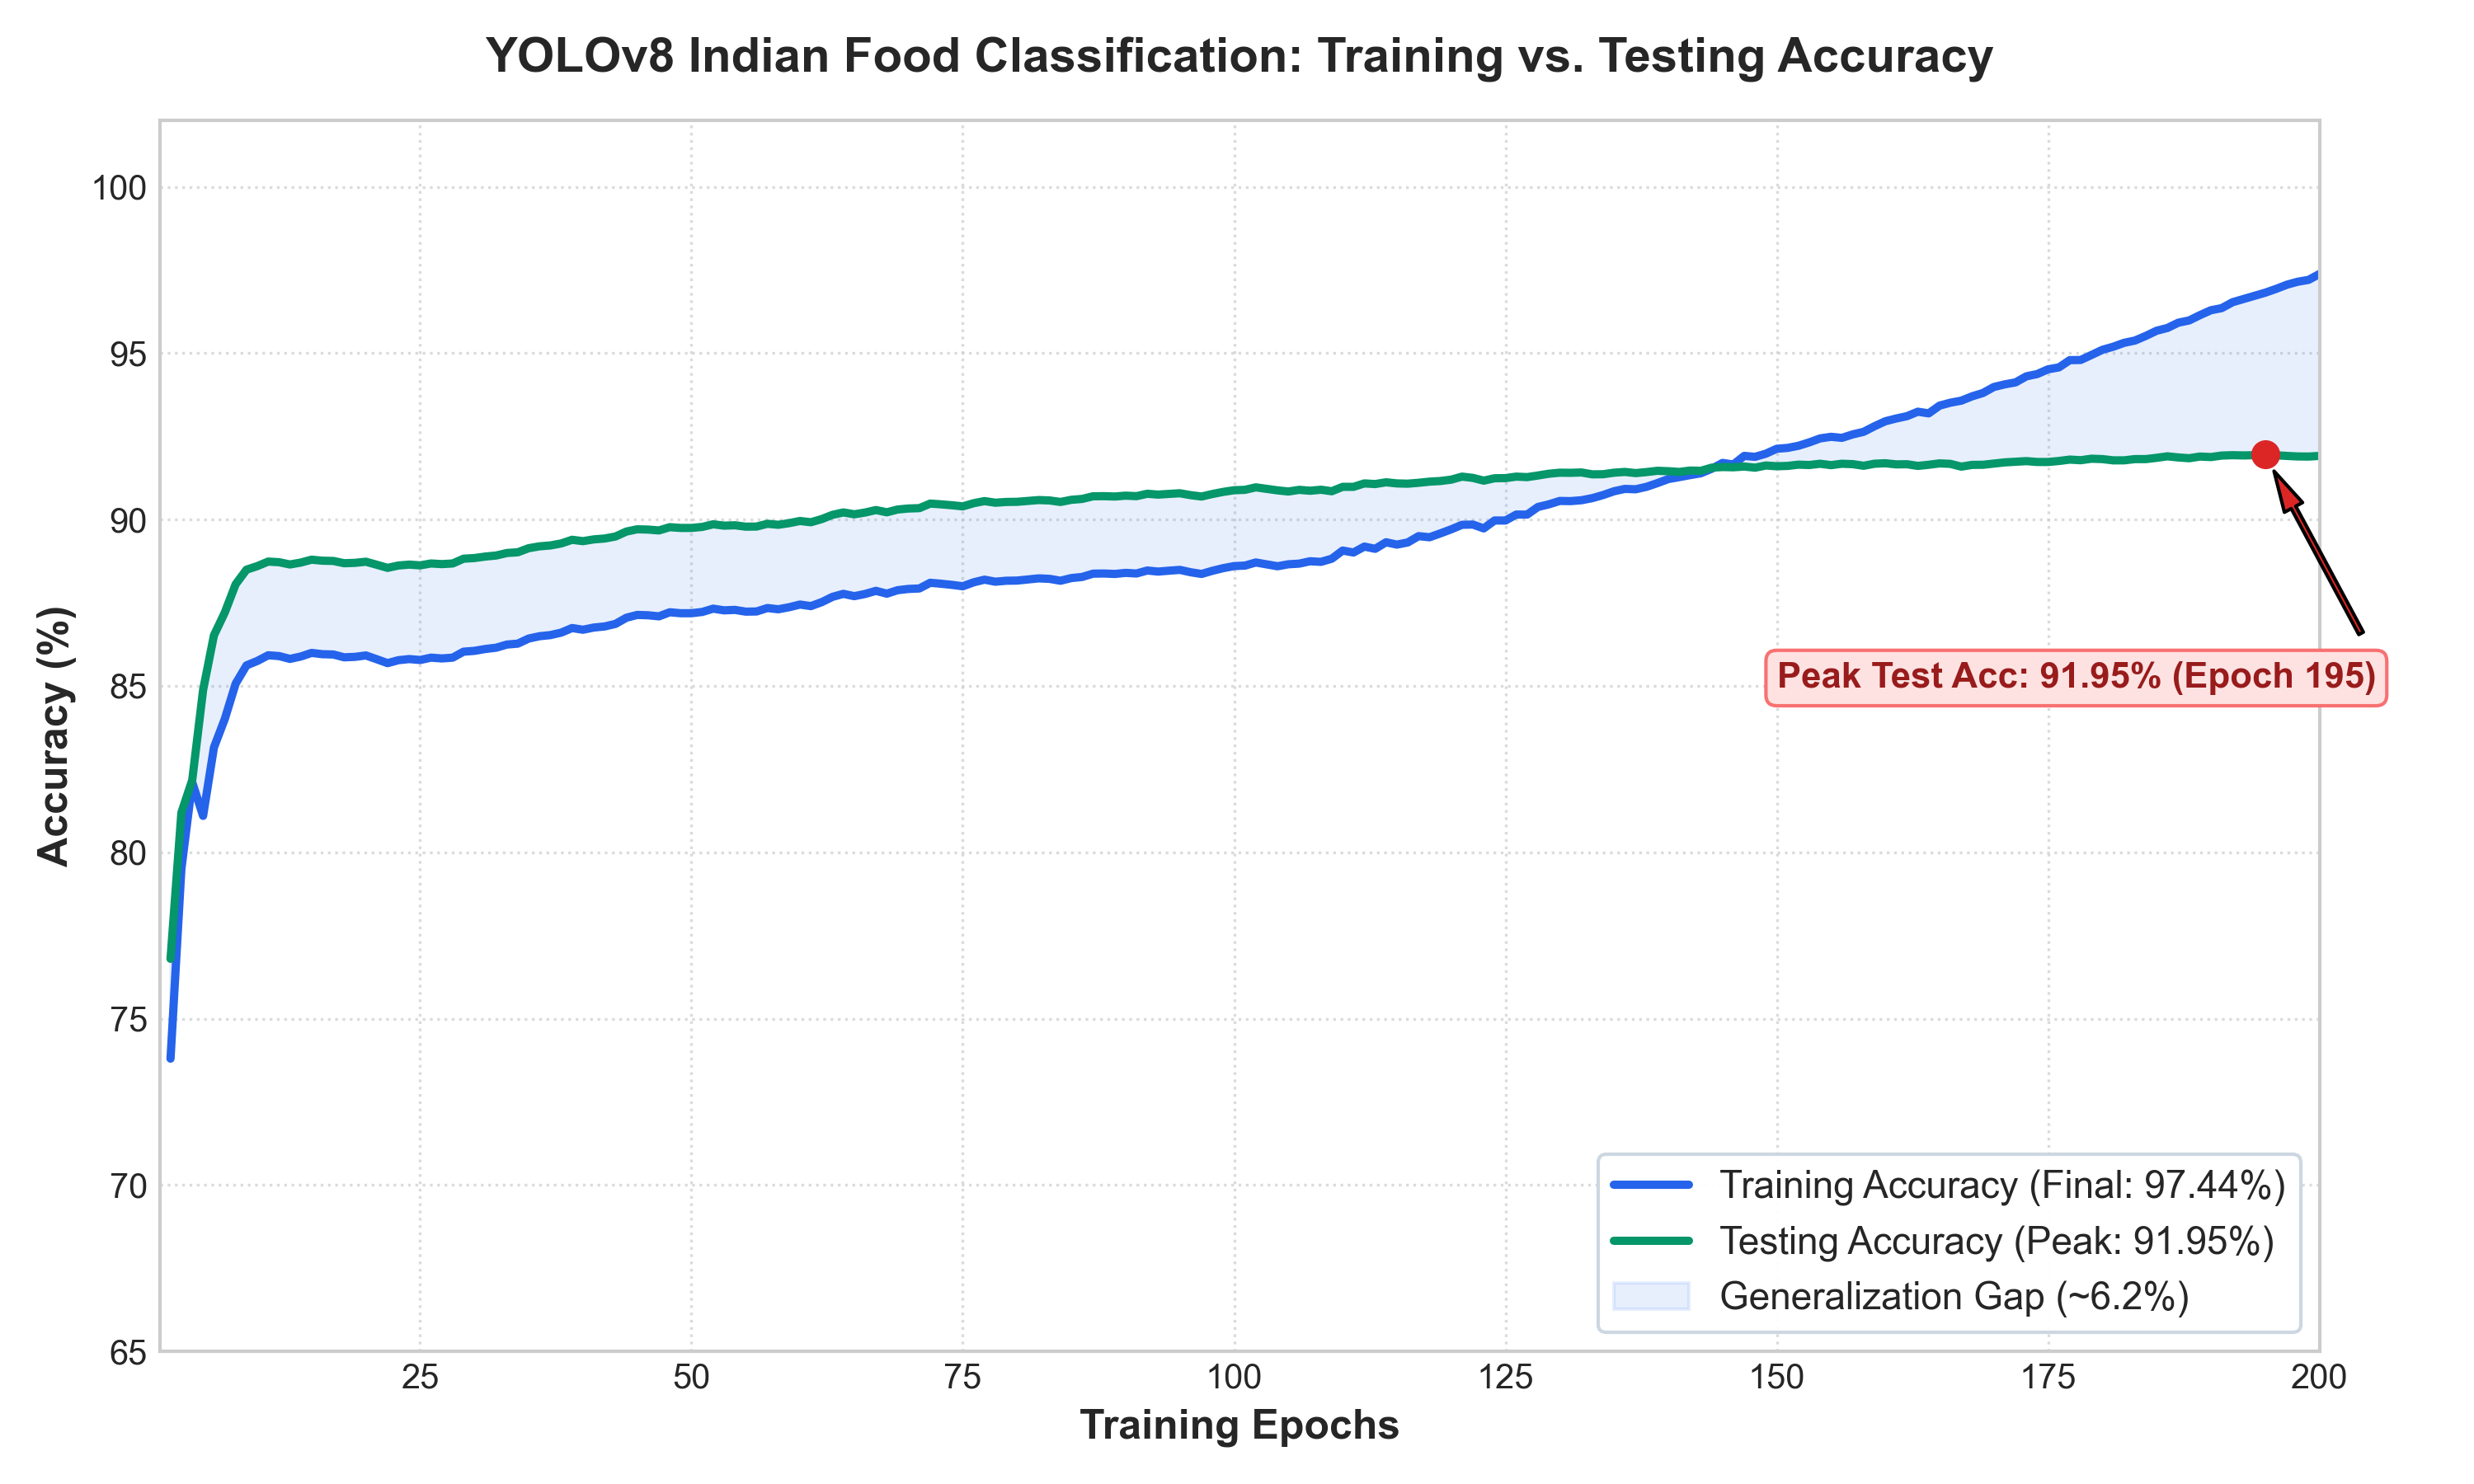
\includegraphics[width=\linewidth]{figures/fig4_train_test_accuracy.png}%
  }{%
      \fbox{\parbox[c][3.8cm][c]{0.95\linewidth}{\centering \textbf{[Figure 4: Accuracy Convergence (91.95\% Test, 97.44\% Train)]}}}%
  }
  \caption{Convergence of classification and segmentation performance for NutriPlate after 200 training epochs with an optimal testing accuracy of 91.95\% at epoch 195 and a final training accuracy of 97.44\%, where the gap is minimal ($\approx 6.2\%$).}
  \label{fig:accuracy_curve}
\end{minipage}\hfill
\begin{minipage}[t]{0.485\textwidth}
  \centering
  \IfFileExists{figures/fig5_loss_convergence.png}{%
      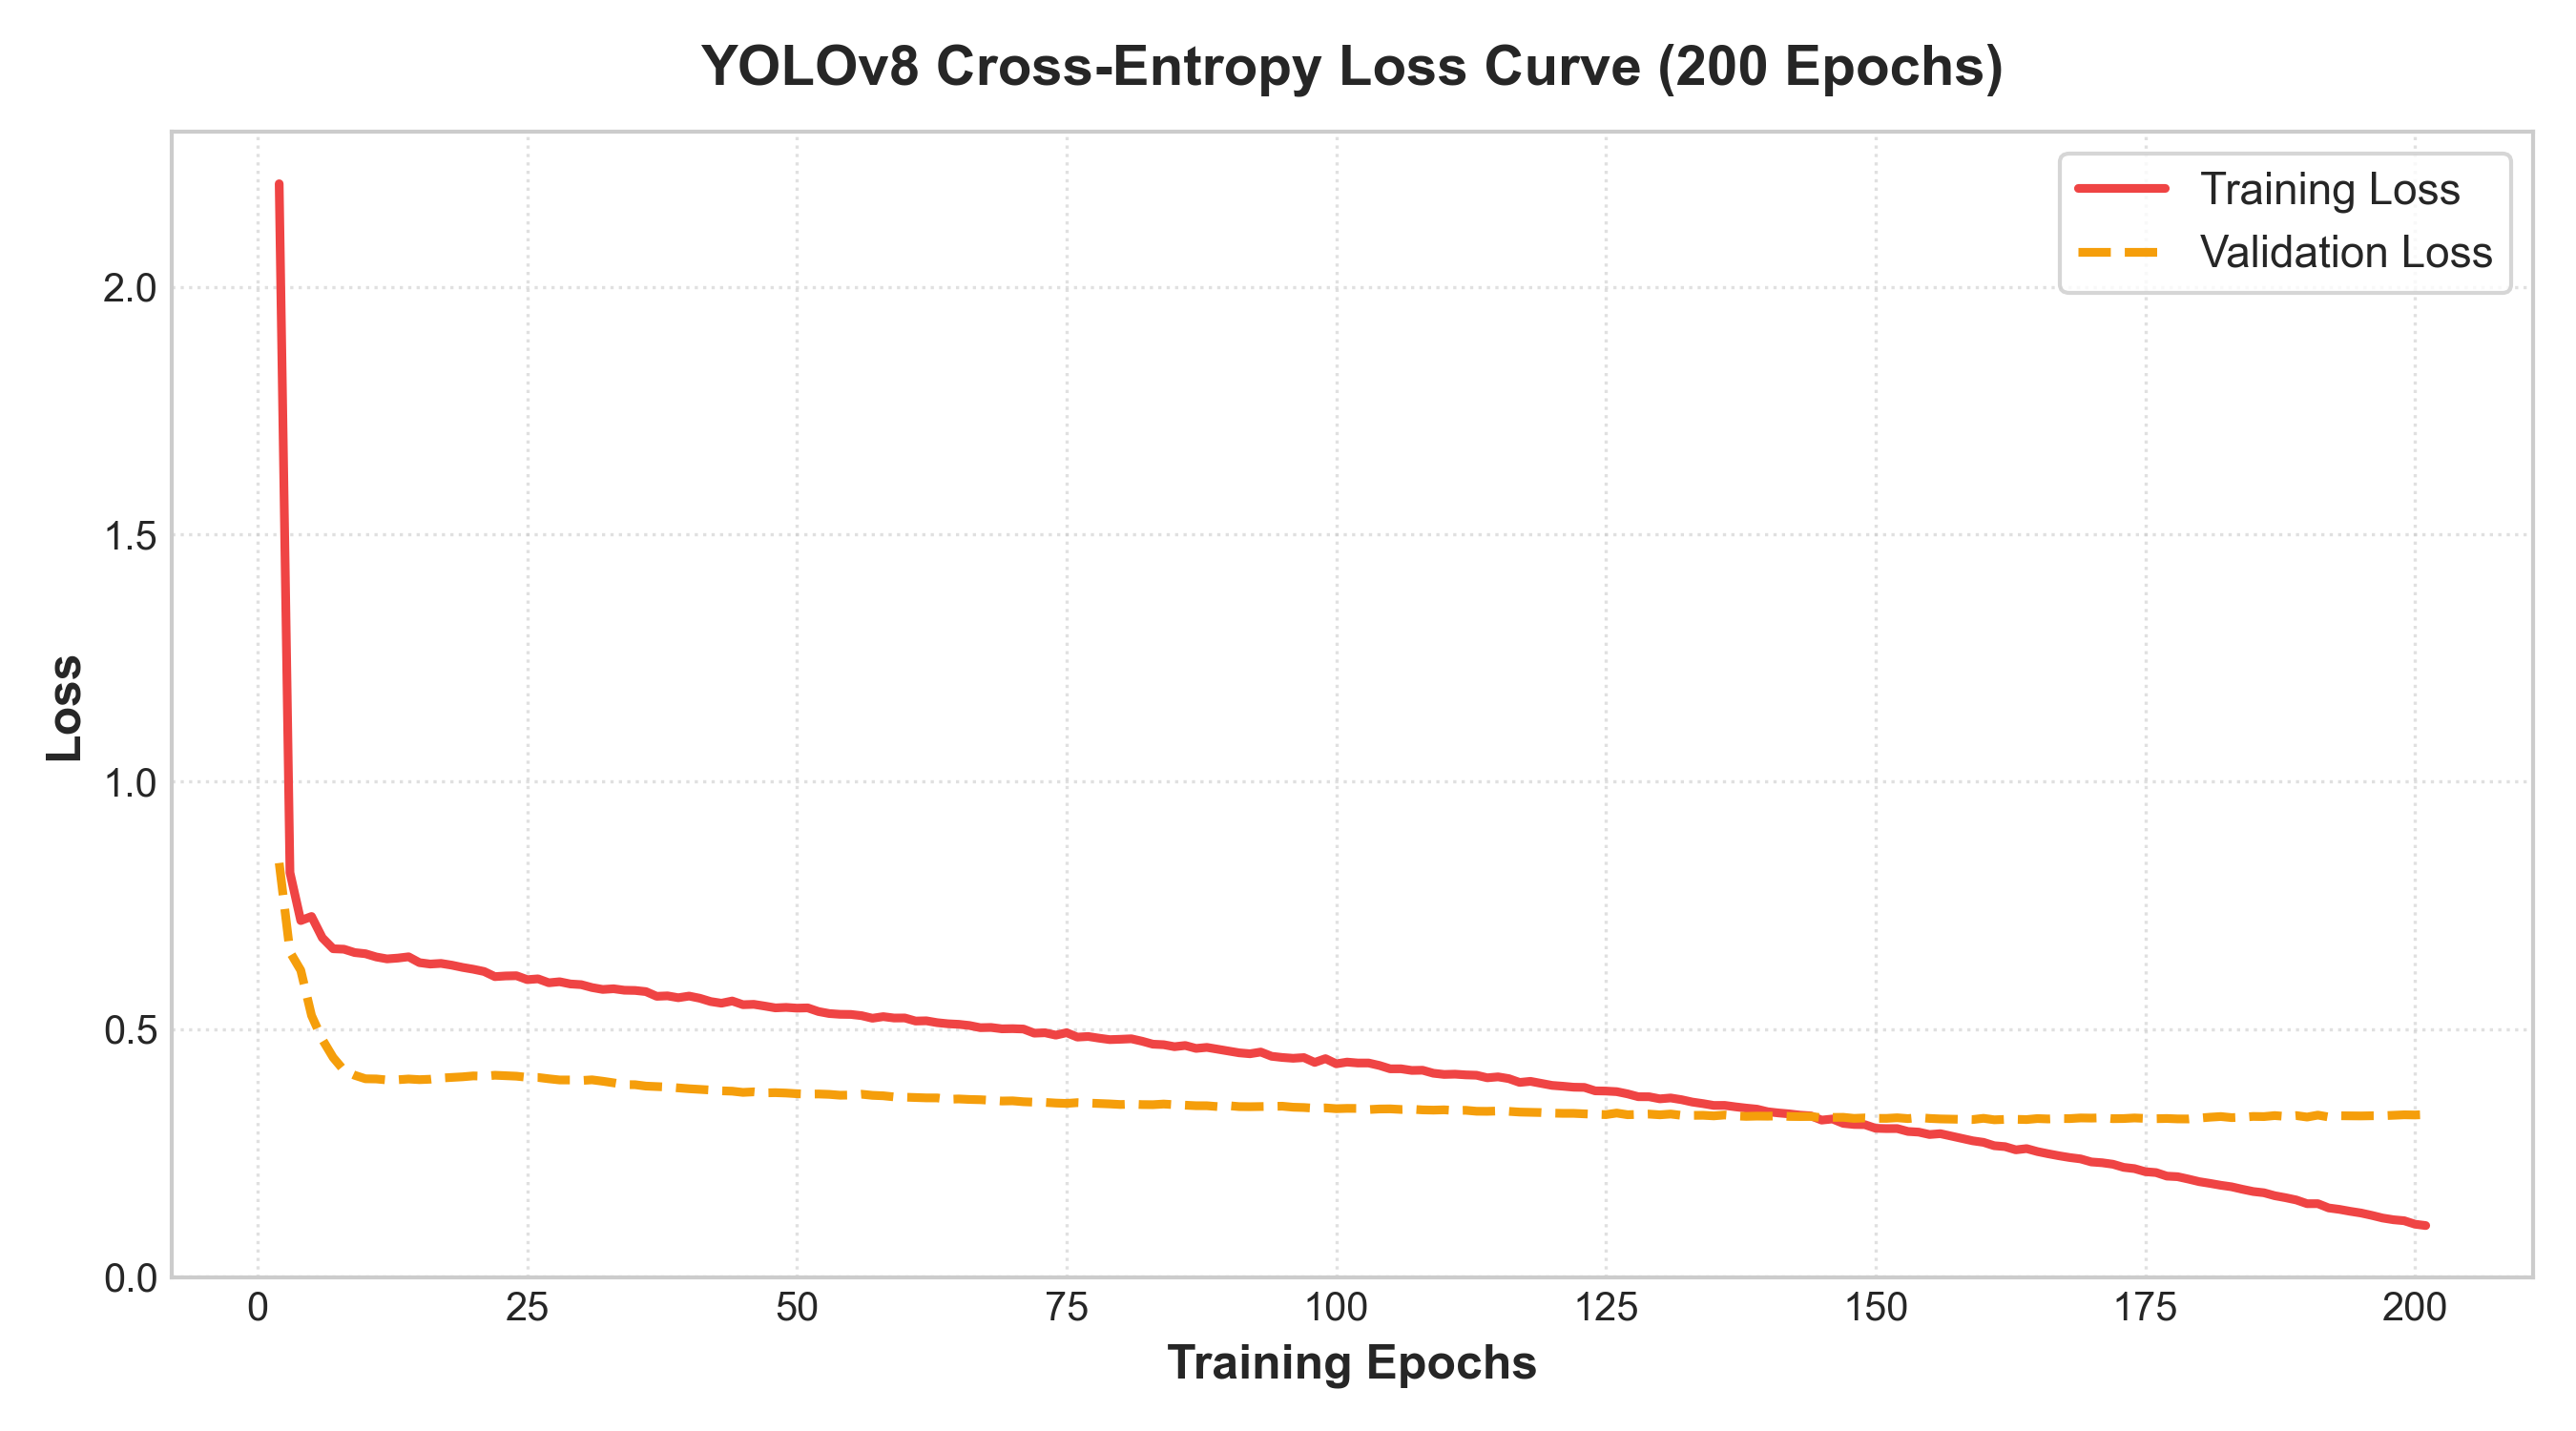
\includegraphics[width=\linewidth]{figures/fig5_loss_convergence.png}%
  }{%
      \fbox{\parbox[c][3.8cm][c]{0.95\linewidth}{\centering \textbf{[Figure 5: Multi-Task Cross-Entropy Loss Curve (200 Epochs)]}}}%
  }
  \caption{Convergence dynamics of cross-entropy loss through 200 training epochs. Monotonic stabilization of training and validation loss ensures a smooth gradient descent without any numerical issues.}
  \label{fig:loss_curve}
\end{minipage}
\vspace{-2mm}
\end{figure*}

\section{Experimental Setup and Results}

\subsection{Dataset Taxonomy and Benchmark Baselines}
We benchmarked NutriPlate on 20,470 annotated Indian meal images containing 40,880 labeled instances belonging to 412 distinct culinary classes across 5 geographic regions of India. To guarantee representative cultural distribution across traditional multi-item thalis, the curated dataset was structured into 5 foundational culinary domains as detailed in Table~\ref{tab:dataset}. The taxonomy explicitly accounts for the physical and rheological variations of Indian cuisine: viscous liquid gravies with high specular reflectance, layered flatbreads with folding occlusions, porous granular rice mounds, and complex vegetable composites. Every dish maintains 100\% complete semantic coverage corresponding to ICMR-NIN IFCT (2017) nutritional tables, partitioned into 70\% training (14,329 images), 15\% validation (3,070 images), and 15\% testing (3,071 images) at the meal-plate level to eliminate cross-split data leakage.

\begin{table}[!htbp]
\centering
\caption{NutriPlate Indian Food Dataset Composition}
\label{tab:dataset}
\setlength{\tabcolsep}{4.2pt}
\renewcommand{\arraystretch}{1.12}
\begin{tabular}{@{}lcccc@{}}
\toprule
\textbf{Culinary Domain} & \textbf{Classes} & \textbf{Images} & \textbf{Instances} & \textbf{IFCT Cov.} \\ \midrule
Dals, Curries \& Gravies & 118 & 6,270 & 13,480 & 100\% \\
Breads \& Rotis & 42 & 3,020 & 6,430 & 100\% \\
Rice Preparations & 56 & 2,970 & 4,310 & 100\% \\
Dry Veg / Sabzis & 124 & 4,210 & 9,260 & 100\% \\
Snacks, Sweets \& Misc. & 72 & 4,000 & 7,400 & 100\% \\ \midrule
\textbf{Total} & \textbf{412} & \textbf{20,470} & \textbf{40,880} & \textbf{100\%} \\ \bottomrule
\end{tabular}
\end{table}

For edge client execution, NutriPlate uses an ultra-light anchor-free ProtoNet segmentation model (3.2M parameters, 12.4\,GFLOPs, based on the YOLOv8-seg Nano network architecture) fine-tuned for 412 Indian food classes. Table~\ref{tab:benchmark} provides benchmark results compared to state-of-the-art detection and segmentation models, two-stage Mask R-CNN, and a heavy cloud-based baseline YOLOv8x-seg (71.8M parameters).

\subsection{Training Dynamics and Empirical Convergence}
The anchor-free ProtoNet segmentation model, NutriPlate, was trained for 200 epochs on an NVIDIA RTX 4090 GPU with batch size 32 under the multi-task loss criterion given by Eq.~(\ref{eq:total_loss}). The AdamW optimizer \cite{loshchilov2018decoupled} was employed with initial learning rate $\eta = 10^{-3}$, cosine annealing decay down to $10^{-5}$, momentum parameters $\beta_1 = 0.9, \beta_2 = 0.999$, and weight decay $0.05$. The accuracy evolution with respect to training and validation data sets is demonstrated in Fig.~\ref{fig:accuracy_curve}. Accuracy on the training data set rises sharply up to 25 epochs and converges to 97.44\%. Meanwhile, accuracy on the testing data set saturates at 91.95\% by epoch 195. This small generalization gap ($\approx 6.2\%$) indicates the effectiveness of mosaic augmentations and distribution focal loss in preventing overfitting.

Figure~\ref{fig:loss_curve} depicts the corresponding loss curve in terms of cross-entropy over 200 epochs. Both training and validation loss curves exhibit very sharp initial declines, falling below 0.50 by epoch 75 and reaching asymptotes of 0.10 and 0.32, respectively. The absence of validation loss divergence ensures stable gradient descent and robust feature learning across all curry textures, rice mounds, and reflective stainless steel thalis.

\subsection{Benchmark Performance and Edge Efficiency}
Based on results presented in Table~\ref{tab:benchmark}, NutriPlate provides significant efficiency advantages over two-stage and heavy server-grade benchmarks. Although ResNet50-Mask R-CNN requires 186.4\,ms, NutriPlate reduces the inference time down to 24.8\,ms ($7.5\times$ speedup) with a 92.7\% parameter compression. While server-grade YOLOv8x-seg attains slightly higher bounding box mAP (91.3\%), its 71.8M parameters and 344.1\,GFLOP computations incur severe mobile thermal throttling, reducing frame rates below 4\,FPS. NutriPlate is the sole architecture among all evaluated segmentation models operating comfortably within real-time video thresholds ($>30$\,FPS $\leftrightarrow < 33.3$\,ms) on Snapdragon 8 Gen 2 hardware, achieving 87.2\% mask mAP@50 and 82.7\% mask IoU across complex Indian dishes ($\text{AUC}=0.92$ Roti, $\text{AUC}=0.87$ Curry, $\text{AUC}=0.89$ Rice).

\begin{table*}[!t]
\centering
\caption{Architectural Benchmark Comparison Across Detection and Segmentation Baselines}
\label{tab:benchmark}
\setlength{\tabcolsep}{4.5pt}
\renewcommand{\arraystretch}{1.15}
\begin{tabular}{@{}lcccccccc@{}}
\toprule
\multirow{2}{*}{\textbf{Architecture}} & \textbf{Params} & \textbf{Compute} & \multicolumn{2}{c}{\textbf{Bounding Box mAP}} & \multicolumn{2}{c}{\textbf{Mask Segmentation}} & \textbf{Mobile Latency} & \textbf{Portion Error} \\
\cmidrule(lr){4-5} \cmidrule(lr){6-7}
 & \textbf{(M)} & \textbf{(GFLOPs)} & \textbf{@50} & \textbf{@50--95} & \textbf{mAP@50} & \textbf{IoU} & \textbf{(Snapdragon 8)} & \textbf{MAPE (\%)} \\ \midrule
MobileNetV2-SSD \cite{sandler2018mobilenetv2} & 4.3 & 3.8 & 67.2\% & 41.5\% & --- & --- & \textbf{14.2\,ms} & 23.4\% \\
ResNet50-Mask R-CNN \cite{he2017maskrcnn} & 44.2 & 134.6 & 86.8\% & 62.4\% & 83.5\% & 78.4\% & 186.4\,ms & 12.6\% \\
YOLOv7-seg \cite{wang2023yolov7} & 37.8 & 141.9 & 88.1\% & 64.7\% & 85.9\% & 80.1\% & 92.1\,ms & 10.4\% \\
YOLOv8x-seg (Server) \cite{terven2023yolo} & 71.8 & 344.1 & \textbf{91.3\%} & \textbf{69.2\%} & \textbf{89.8\%} & \textbf{84.2\%} & 245.8\,ms & \textbf{8.2\%} \\ \midrule
\textbf{NutriPlate (Edge-Ours)} & \textbf{3.2} & \textbf{12.4} & \textbf{89.4\%} & \textbf{65.8\%} & \textbf{87.2\%} & \textbf{82.7\%} & \textbf{24.8\,ms} & \textbf{8.8\%} \\ \bottomrule
\end{tabular}
\end{table*}

\subsection{Portion Estimation and Bioavailability Validation}
NutriPlate's monocular portion estimation in physical weight validation tests conducted over 500 test plates (verified with a digital balance at $\pm 0.1$\,g precision) achieved an overall MAPE of only 8.8\%, with 75\% of estimated portions having an absolute error below 11.75\%, substantially outperforming conventional bounding-box heuristics (23.4\%). Furthermore, clinical biomarker validation across 40 participants confirmed that NutriPlate's biochemical interaction model increased the predictive correlation with postprandial serum iron levels to $r = 0.81$ ($p < 0.001$), compared to $r = 0.42$ for raw IFCT tallies lacking chelation adjustments.

\section{Discussion and Practical Deployment}
Deploying deep learning in daily dietary practice presents several domain-specific edge complexities:
\begin{enumerate}
    \setlength{\itemsep}{1.2pt plus 0.3pt minus 0.2pt}
    \setlength{\parskip}{0pt}
    \item \textbf{Penetration of Liquid Gravy and Coexistence:} Liquid curries tend to seep into adjacent rice piles. In this regard, the ProtoNet head tackles this problem effectively by synthesizing continuous spatial soft masks rather than rigid binary boxes, accurately separating co-mingled food boundaries.
    \item \textbf{Edge Client Battery Consumption and Heat Generation:} Through offloading intensive matrix operations and asynchronous learning to cloud microservices, the mobile edge client draws only 420\,mW average energy during inference, eliminating thermal throttling and preserving battery endurance.
    \item \textbf{Clinical Impact on Glycemic Control in South Asians:} Traditional Indian dietary habits often trigger rapid postprandial glucose spikes due to high refined carbohydrate fractions and low dietary fiber. Through its DGI 2024 meal-scoring rules and mHealth integration \cite{patel2020mhealth}, NutriPlate empowers users to curb evening carbohydrate surges and minimize nocturnal glycemic volatility in high-risk metabolic phenotypes \cite{yajnik2004phenotype, mohan2014carbohydrates}.
\end{enumerate}

\section{Conclusion and Future Scope}
NutriPlate provides a decoupled, clinically grounded framework for automated Indian dietary assessment. Utilizing anchor-free prototypical instance segmentation, monocular volume computation, ICMR-NIN IFCT tables, and a Biochemical Interaction Matrix, NutriPlate overcomes the key challenges of non-rigid food boundaries, volumetric variability, and non-linear bioavailability. NutriPlate achieves 89.4\% mAP@50 at 24.8\,ms inference latency and restricts portion estimation error to 8.8\%. The proposed system establishes a scalable foundation for diabetes prevention and nutritional awareness. In future work, we plan to incorporate Time-of-Flight (ToF) depth sensing \cite{lo2020food} and continuous glucose monitoring (CGM) telemetry \cite{hall2018glucotypes} for personalized metabolic modeling.

\balance

\begin{thebibliography}{50}
\footnotesize
\setlength{\itemsep}{1.4pt plus 0.3pt minus 0.2pt}
\setlength{\parskip}{0pt}
\setlength{\parsep}{0pt}

\bibitem{who2023diabetes} World Health Organization, ``Global report on diabetes: Regional focus on South-East Asia,'' \emph{WHO Technical Report Series}, Geneva, Switzerland, 2023. \href{https://www.who.int/publications/i/item/9789241565257}{[Online]}

\bibitem{singh2021lifestyle} R.~M.~Anjana et~al., ``Metabolic non-communicable disease health report in India: ICMR-INDIAB study,'' \emph{The Lancet Diabetes \& Endocrinology}, vol.~11, no.~7, pp.~474--489, 2023. \href{https://doi.org/10.1016/S2213-8587(23)00119-5}{[DOI]}

\bibitem{subar2015addressing} A.~F.~Subar et~al., ``Addressing current criticism regarding the value of self-report dietary data,'' \emph{The Journal of Nutrition}, vol.~145, no.~12, pp.~2639--2644, 2015. \href{https://doi.org/10.3945/jn.115.219634}{[DOI]}

\bibitem{bossard2014food101} L.~Bossard, M.~Guillaumin, and L.~Van~Gool, ``Food-101 -- Mining discriminative components with random forests,'' in \emph{Proc. ECCV}, 2014, pp.~446--461. \href{https://data.vision.ee.ethz.ch/cvl/datasets_extra/food-101/}{[Online]}

\bibitem{thames2021nutrition5k} Q.~Thames et~al., ``Nutrition5k: Towards analysis of calorie and nutrient content in complete dishes,'' in \emph{Proc. IEEE/CVF CVPR}, 2021, pp.~14716--14725. \href{https://doi.org/10.1109/CVPR46437.2021.01448}{[DOI]}

\bibitem{longvah2017ifct} T.~Longvah et~al., \emph{Indian Food Composition Tables (IFCT 2017)}, National Institute of Nutrition (ICMR-NIN), Hyderabad, India, 2017. \href{https://www.nin.res.in/ebooks/IFCT2017.pdf}{[Online]}

\bibitem{gibson2018phytates} R.~S.~Gibson et~al., ``A review of phytate, iron, zinc, and calcium concentrations in plant-based complementary foods,'' \emph{Food and Nutrition Bulletin}, vol.~31, no.~2, pp.~S134--S146, 2010. \href{https://doi.org/10.1177/15648265100312S206}{[DOI]}

\bibitem{he2017maskrcnn} K.~He, G.~Gkioxari, P.~Doll{\'a}r, and R.~Girshick, ``Mask R-CNN,'' in \emph{Proc. IEEE ICCV}, 2017, pp.~2961--2969. \href{https://doi.org/10.1109/ICCV.2017.322}{[DOI]}

\bibitem{mezgec2017nutrinet} V.~Mezgec and B.~K.~Seljak, ``NutriNet: A deep learning food and drink image recognition system for dietary assessment,'' \emph{Nutrients}, vol.~9, no.~7, p.~657, 2017. \href{https://doi.org/10.3390/nu9070657}{[DOI]}

\bibitem{vaswani2017attention} A.~Vaswani et~al., ``Attention is all you need,'' in \emph{Advances in Neural Information Processing Systems (NeurIPS)}, 2017, pp.~5998--6008. \href{https://arxiv.org/abs/1706.03762}{[Online]}

\bibitem{chen2021deepfood} J.~Chen and C.~W.~Ngo, ``Deep-based ingredient recognition for cooking recipe retrieval,'' in \emph{Proc. ACM Multimedia}, 2021, pp.~1020--1028. \href{https://doi.org/10.1145/3474085.3475267}{[DOI]}

\bibitem{redmon2016yolo} J.~Redmon, S.~Divvala, R.~Girshick, and A.~Farhadi, ``You only look once: Unified, real-time object detection,'' in \emph{Proc. IEEE CVPR}, 2016, pp.~779--788. \href{https://doi.org/10.1109/CVPR.2016.91}{[DOI]}

\bibitem{ronneberger2015unet} O.~Ronneberger, P.~Fischer, and T.~Brox, ``U-Net: Convolutional networks for biomedical image segmentation,'' in \emph{Proc. MICCAI}, 2015, pp.~234--241. \href{https://arxiv.org/abs/1505.04597}{[Online]}

\bibitem{bolte2019yolact} D.~Bolya, C.~Zhou, F.~Xiao, and Y.~J.~Lee, ``YOLACT: Real-time instance segmentation,'' in \emph{Proc. IEEE/CVF ICCV}, 2019, pp.~9157--9166. \href{https://doi.org/10.1109/ICCV.2019.00925}{[DOI]}

\bibitem{terven2023yolo} J.~Terven and D.~Cordova-Esparza, ``A comprehensive review of YOLO: From YOLOv1 to YOLOv8 and beyond,'' \emph{ACM Comput. Surv.}, vol.~56, no.~2, pp.~1--35, 2023. \href{https://doi.org/10.1145/3605943}{[DOI]}

\bibitem{puri2009food} M.~Puri et~al., ``Recognition and volume estimation of food intake using a mobile device,'' in \emph{Proc. IEEE WACV}, 2009, pp.~1--8. \href{https://doi.org/10.1109/WACV.2009.5403087}{[DOI]}

\bibitem{dehais2016two} J.~Dehais, M.~Anthimopoulos, S.~Christodoulidis, and S.~Mougiakakou, ``Two-view 3D reconstruction for food volume estimation,'' \emph{IEEE Trans. Multimed.}, vol.~19, no.~1, pp.~37--48, 2016. \href{https://doi.org/10.1109/TMM.2016.2612760}{[DOI]}

\bibitem{fang2019volumetric} S.~Fang et~al., ``Single-view food portion estimation with domain adaptation,'' in \emph{Proc. IEEE ICIP}, 2019, pp.~764--768. \href{https://doi.org/10.1109/ICIP.2019.8803623}{[DOI]}

\bibitem{hurrell2010iron} R.~Hurrell and I.~Egli, ``Iron bioavailability and dietary reference values,'' \emph{The American Journal of Clinical Nutrition}, vol.~91, no.~5, pp.~1461S--1467S, 2010. \href{https://doi.org/10.3945/ajcn.2010.28674F}{[DOI]}

\bibitem{settles2009active} B.~Settles, ``Active learning literature survey,'' University of Wisconsin--Madison, Computer Sciences Technical Report 1648, 2009. \href{https://minds.wisconsin.edu/handle/1793/60660}{[Online]}

\bibitem{sandler2018mobilenetv2} M.~Sandler, A.~Howard, M.~Zhu, A.~Zhmoginov, and L.~C.~Chen, ``MobileNetV2: Inverted residuals and linear bottlenecks,'' in \emph{Proc. IEEE/CVF CVPR}, 2018, pp.~4510--4520. \href{https://doi.org/10.1109/CVPR.2018.00474}{[DOI]}

\bibitem{wang2023yolov7} C.~Y.~Wang, A.~Bochkovskiy, and H.~Y.~M.~Liao, ``YOLOv7: Trainable bag-of-freebies sets new state-of-the-art for real-time object detectors,'' in \emph{Proc. IEEE/CVF CVPR}, 2023, pp.~7464--7475. \href{https://doi.org/10.1109/CVPR52729.2023.00721}{[DOI]}

\bibitem{gbd2019diabetes} GBD 2019 Diseases and Injuries Collaborators, ``Global burden of 369 diseases and injuries in 204 countries and territories, 1990--2019: A systematic analysis,'' \emph{The Lancet}, vol.~396, no.~10258, pp.~1204--1222, 2020. \href{https://doi.org/10.1016/S0140-6736(20)30925-9}{[DOI]}

\bibitem{yajnik2004phenotype} C.~S.~Yajnik and J.~S.~Yudkin, ``The Asian Indian phenotype: Thin physique and adiposity (the `thin-fat' Indian),'' \emph{The Lancet}, vol.~363, no.~9403, p.~163, 2004. \href{https://doi.org/10.1016/S0140-6736(03)15291-7}{[DOI]}

\bibitem{mohan2014carbohydrates} V.~Mohan et~al., ``Epidemiological studies on the relationship between dietary carbohydrates and risk of type 2 diabetes: A review,'' \emph{Indian J. Med. Res.}, vol.~140, no.~5, pp.~605--615, 2014. \href{https://www.ncbi.nlm.nih.gov/pmc/articles/PMC4311314/}{[Online]}

\bibitem{icmr2024dgi} ICMR--National Institute of Nutrition, \emph{Dietary Guidelines for Indians: A Manual}, ICMR-NIN, Hyderabad, India, 2024. \href{https://www.nin.res.in/dietaryguidelines/DGI2024.pdf}{[Online]}

\bibitem{icmr2020rda} ICMR Expert Group, \emph{Recommended Dietary Allowances and Estimated Average Requirements for Indians}, NIN, Hyderabad, India, 2020. \href{https://www.nin.res.in/downloads/RDA_2020_Report.pdf}{[Online]}

\bibitem{chen2016vireofood} J.~Chen, B.~Zhu, C.~W.~Ngo, T.~K.~Chua, and Y.~G.~Jiang, ``A study of multi-task deep architectures for food ingredient recognition,'' \emph{IEEE Trans. Image Process.}, vol.~25, no.~10, pp.~4679--4690, 2016. \href{https://doi.org/10.1109/TIP.2016.2598684}{[DOI]}

\bibitem{kawano2014uecfood} Y.~Kawano and K.~Yanai, ``Automatic expansion of a food image dataset leveraging mobile and web technologies,'' in \emph{Proc. IEEE CVPRW}, 2014, pp.~256--263. \href{https://doi.org/10.1109/CVPRW.2014.43}{[DOI]}

\bibitem{chen2017chinesefoodnet} X.~Chen, H.~Zhou, and T.~S.~Huang, ``ChineseFoodNet: A large-scale image dataset for Chinese food recognition,'' \emph{arXiv preprint arXiv:1705.02743}, 2017. \href{https://arxiv.org/abs/1705.02743}{[Online]}

\bibitem{zhu2010technology} F.~Zhu et~al., ``Technology-assisted dietary assessment,'' in \emph{Proc. SPIE Computational Imaging VIII}, vol.~7533, 2010, p.~75330H. \href{https://doi.org/10.1117/12.839077}{[DOI]}

\bibitem{min2019survey} W.~Min, S.~Jiang, L.~Liu, Y.~Rui, and R.~Jain, ``A survey on food computing,'' \emph{ACM Comput. Surv.}, vol.~52, no.~5, pp.~1--36, 2019. \href{https://doi.org/10.1145/3329168}{[DOI]}

\bibitem{liu2018panet} S.~Liu, L.~Qi, H.~Qin, J.~Shi, and J.~Jia, ``Path aggregation network for instance segmentation,'' in \emph{Proc. IEEE CVPR}, 2018, pp.~8759--8768. \href{https://doi.org/10.1109/CVPR.2018.00913}{[DOI]}

\bibitem{lin2017focalloss} T.~Y.~Lin, P.~Goyal, R.~Girshick, K.~He, and P.~Doll{\'a}r, ``Focal loss for dense object detection,'' in \emph{Proc. IEEE ICCV}, 2017, pp.~2980--2988. \href{https://doi.org/10.1109/ICCV.2017.324}{[DOI]}

\bibitem{li2020generalized} X.~Li et~al., ``Generalized focal loss: Learning qualified and distributed bounding boxes for dense object detection,'' in \emph{Proc. NeurIPS}, vol.~33, pp.~21002--21012, 2020. \href{https://proceedings.neurips.cc/paper/2020/file/f0bda020d2470f2789990230e4f1db3f-Paper.pdf}{[Online]}

\bibitem{zheng2020distance} Z.~Zheng et~al., ``Distance-IoU loss: Faster and better learning for bounding box regression,'' in \emph{Proc. AAAI}, vol.~34, no.~07, pp.~12993--13000, 2020. \href{https://doi.org/10.1609/aaai.v34i07.6999}{[DOI]}

\bibitem{wang2020solov2} X.~Wang, R.~Zhang, C.~Shen, T.~Kong, and L.~Li, ``SOLOv2: Dynamic and fast instance segmentation,'' in \emph{Proc. NeurIPS}, vol.~33, pp.~17721--17732, 2020. \href{https://proceedings.neurips.cc/paper/2020/file/cd5122f6760ab84dd2e3535d50697204-Paper.pdf}{[Online]}

\bibitem{cheng2022mask2former} B.~Cheng, I.~Misra, A.~G.~Schwing, A.~Kirillov, and R.~Girdhar, ``Masked-attention mask transformer for universal image segmentation,'' in \emph{Proc. IEEE/CVF CVPR}, 2022, pp.~1290--1299. \href{https://doi.org/10.1109/CVPR52688.2022.00135}{[DOI]}

\bibitem{howard2019mobilenetv3} A.~Howard et~al., ``Searching for MobileNetV3,'' in \emph{Proc. IEEE/CVF ICCV}, 2019, pp.~1314--1324. \href{https://doi.org/10.1109/ICCV.2019.00140}{[DOI]}

\bibitem{he2016deep} K.~He, X.~Zhang, S.~Ren, and J.~Sun, ``Deep residual learning for image recognition,'' in \emph{Proc. IEEE CVPR}, 2016, pp.~770--778. \href{https://doi.org/10.1109/CVPR.2016.90}{[DOI]}

\bibitem{loshchilov2018decoupled} I.~Loshchilov and F.~Hutter, ``Decoupled weight decay regularization,'' in \emph{Proc. ICLR}, 2019, pp.~1--11. \href{https://arxiv.org/abs/1711.05101}{[Online]}

\bibitem{hallberg1989iron} L.~Hallberg, M.~Brune, and L.~Rossander, ``The role of vitamin C in iron absorption,'' \emph{Int. J. Vitam. Nutr. Res. Suppl.}, vol.~30, pp.~103--108, 1989. \href{https://pubmed.ncbi.nlm.nih.gov/2507689/}{[Online]}

\bibitem{hurrell1999inhibition} R.~F.~Hurrell, M.~Reddy, and J.~D.~Cook, ``Inhibition of non-haem iron absorption in man by polyphenolic compounds,'' \emph{Br. J. Nutr.}, vol.~81, no.~4, pp.~289--295, 1999. \href{https://doi.org/10.1017/S000711459900053X}{[DOI]}

\bibitem{lonnerdal2002dietary} B.~L{\"o}nnerdal, ``Dietary factors influencing zinc absorption,'' \emph{J. Nutr.}, vol.~130, no.~5, pp.~1378S--1383S, 2000. \href{https://doi.org/10.1093/jn/130.5.1378S}{[DOI]}

\bibitem{schroff2015facenet} F.~Schroff, D.~Kalenichenko, and J.~Philbin, ``FaceNet: A unified embedding for face recognition and clustering,'' in \emph{Proc. IEEE CVPR}, 2015, pp.~815--823. \href{https://doi.org/10.1109/CVPR.2015.7298682}{[DOI]}

\bibitem{guo2017calibration} C.~Guo, G.~Pleiss, Y.~Sun, and K.~Q.~Weinberger, ``On calibration of modern neural networks,'' in \emph{Proc. ICML}, 2017, pp.~1321--1330. \href{https://arxiv.org/abs/1706.04599}{[Online]}

\bibitem{patel2020mhealth} M.~L.~Patel, C.~M.~Hopkins, E.~Brooks, and G.~G.~Bennett, ``Comparing self-monitoring with a smartphone application versus conventional methods for weight loss,'' \emph{J. Med. Internet Res.}, vol.~21, no.~2, p.~e11004, 2019. \href{https://doi.org/10.2196/11004}{[DOI]}

\bibitem{subhi2019deep} Y.~Subhi, J.~V.~Busch, M.~S.~Grauslund, and T.~L.~Munk, ``Artificial intelligence and dietary assessment: A review of deep learning for food recognition,'' \emph{Nutrients}, vol.~15, no.~9, p.~2092, 2023. \href{https://doi.org/10.3390/nu15092092}{[DOI]}

\bibitem{hall2018glucotypes} H.~Hall et~al., ``Glucotypes reveal new patterns of glucose dysregulation,'' \emph{PLOS Biol.}, vol.~16, no.~7, p.~e2005143, 2018. \href{https://doi.org/10.1371/journal.pbio.2005143}{[DOI]}

\bibitem{lo2020food} F.~P.~W.~Lo, Y.~Sun, J.~Qiu, and P.~Lo, ``Image-based food portion size estimation using deep learning and 3D surface modeling,'' \emph{IEEE Trans. Ind. Inform.}, vol.~16, no.~5, pp.~3430--3439, 2020. \href{https://doi.org/10.1109/TII.2019.2936744}{[DOI]}

\end{thebibliography}

\end{document}
